\chapter{Prototyping}

% Introduction:
This chapter describes the development and testing of three prototypes. Following the details of each iteration is an analysis of the primary findings.

% Literature Review:
% Auslander, 1999: Communities are formed based on how the audience interacts, with no dependence on the spectacle at hand
% Turino, 2008:
% * Artists can shift between participatory and presentational performance
% * Different roles of different difficult allow for everyone to feel welcome and achieve flow. "Core" and "elaboration" roles cater to advanced and non-advanced performers respectively.
% * Open form: Basic motives repeated over and over. Easy for newcomers to join in. "Security in constancy." Can facilitate flow.
% * Hall: Repetition can increase intensity. Synchronicity comforts people.
% * Wide tuning, loud volumes, and overlapping textures provide a ``cloaking function'' that makes people more comfortable participating
% * Virtuosic solos are not common
% * Some participatory performances are sequential -- everyone gets a turn (e.g. Karaoke)
% Kelly, 2007: Displaying clips and themes from her music videos at a Madonna concert creates feelings of a "shared past" in the audience. (How might we create instead a "shared present"?)
% Small, 1998: Performers dressing in uniform are separating themselves and their responsibilities
% Davidson, 1997:
% * Performance etiquette is usually formed by crowd mentality, following the majority
% * Performers pick up information from the audience's broad and specific behaviours
% * Visuals help audiences read the performer's intentions
% Sexton, 2007: Simple synchronous interactions in sound art projects left users with little to explore, resulting in a "flat" experience
% Jourdain, 1997: We move to music in order to "represent" it. This also amplifies, resonates the musical experience.
% Levitin, 2006:
% * "In every society of which we're aware, music and dance are inseparable." Ancient music was based on rhythm and movement. Combining rhythm and melody bridges our cerebellum and cerebral cortex.
% * Ties between music and movement have only been minimized in the last 100 years
% Kelly, 2007: Technology incorporated into a show can either be addressed as part of the show or hidden and made illusory
% Maynes-Aminzade, 2002:
% * Computer vision: Movement-based control were intuitive, but camera required frequent calibration
% * Beach ball: Using a single beach ball as an input was also intuitive, but it only involved a few people at a time
% * Laser pointers: Gave everyone an individual cursor, but got chaotic once more and more people joined
% * Recommendations: Focus on compelling activity over impressive technology. Not everyone must be sensed as long as they feel involved. The control mechanism should be obvious or the users will give up. Make the activity emotionally engaging. Emphasize cooperation.
% Ulyate, 2001:
% * Design guidelines:
% * * Encourage and reward movement
% * * Feedback should be immediate, obvious, and meaningful in the context of the space
% * * No instruction or thinking should be required
% * * Responsiveness is more important than aesthetics
% * *  Modularity is key
% * Lessons learned:
% * * Full-body movement is most satisfying
% * * Form of the object determines how users interact
% * * A practical system is distributed and scalable
% * * Find balance between freedom and constraint
% * * Users will always find a way to create unwanted outputs
% * * Simple, instant gratification is important for feedback
% Feldmeier, 2007:
% * Crowd had a tendency to gradually move in sync
% Barkhuus, 2008:
% * Inputs based on already-present behaviour lead to intuitive systems
% * Don't focus on employing cutting edge technology
% * Events should not rely on the success of the technology
% * Immediate visual or aural feedback is key
% Tseng, 2012: Being excluded from the interaction did not lessen enjoyment of the show
% Gates, 2006: Technologies should reflect the performer's art and not be a burden on them

\section{Prototype \#1}

% Motivation:
The first prototype served as an initial experiment for investigating how technology might be used to give an audience new means of participating in a performance. My goal was to develop a simple system that featured a single user `performing' -- creating some sort of stimulating output. Multiple `audience members' would then be given the ability to collectively contribute to this output in some way, illustrating a slight shift from presentational to participatory. The prototype was designed to be presented and demoed at a research colloquium. Thus, in addition to being able to observe users' responses to the system, discussion would be stimulated amongst attendees as well.

% Prototype #1 Goals:
% * Exploratory: How might an audience become a part of a performance?

\subsection{Development}

In order to simulate this scenario and avoid having to recruit a rock band for this small experiment, I developed a basic VJ system. VJing is the real-time creation or manipulation of visuals, which are typically projected to accompany music. Thus, the performing user would be controlling projected visuals, and the audience members would be able to manipulate some aspect of them. Having the collective output clearly displayed on one screen would provide the performer and audience members with feedback from their inputs and allow for straightforward observations of their interactions.

The first step in realizing this initial prototype was deciding on the hardware and software that would be used. Wii video game controllers have an abundance of sensors: they contain eleven digital buttons, an infrared sensor, an accelerometer, and (in the newer Wii Remote Plus models) a gyroscope, and all of this data can be sent wirelessly to a receiver via Bluetooth. In addition to these affordances, due to the console's popularity, the Wii controller is also something that many people have used before. With these considerations, I decided that the Wii controller was a suitable input device for my experiment. Figure \ref{prototyping1.6} pictures one of these controllers.
% Argue against smartphones? Ethnography: They could get damaged; they could be distracting. Tomitsch et al.: A diverse audience means diverse technical skills.

\begin{figure}
	\centering

	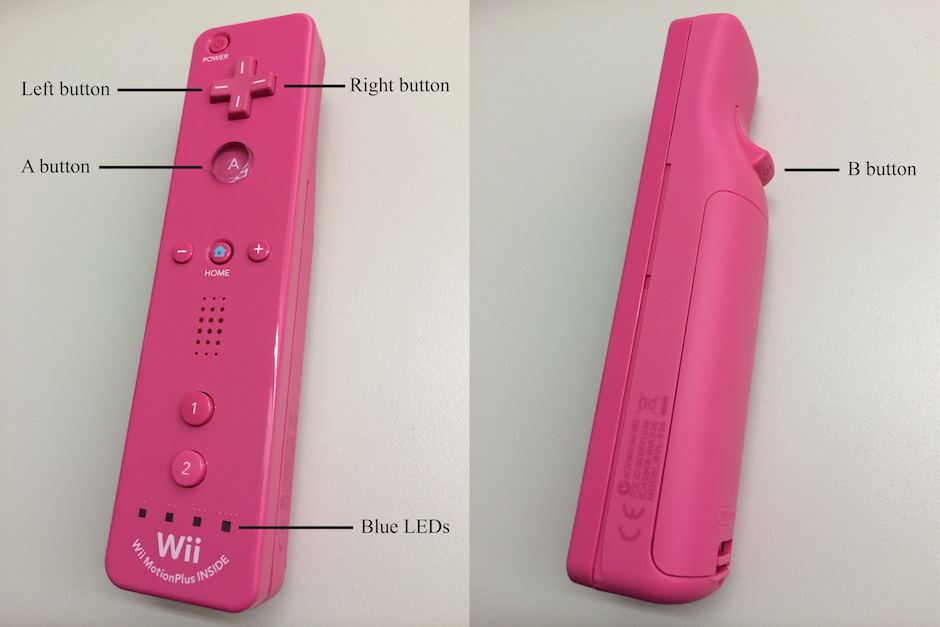
\includegraphics[height=0.4\textwidth]{wii_labelled.png}
	\caption{Wii controller}

	\label{prototyping1.6}
\end{figure}

For my purposes, the easiest way to process the Wii controllers' data was using a combination of two software packages -- OSCulator\footnote{\url{http://www.osculator.net}} and Max\footnote{\url{http://cycling74.com}}. OSCulator allows for communication between devices and audio or video software using the Open Sound Control (OSC) protocol\footnote{\url{http://opensoundcontrol.org}}. Fortunately, this software is also specifically designed to communicate with the Wii controller. It can display live data from each sensor as well as activate the controller's LEDs and rumble motor. The data can then be sent to Max, a visual programming environment that is especially useful for handling multimedia. Countless objects can be incorporated into a Max program (called a `patcher') to manipulate numbers, audio signals, and video clips. Max is commonly used by musicians and video artists to create highly customized and interactive programs; for instance, this software was used in Freeman's (2005) \textit{Glimmer} project.

\begin{figure}
	\centering

	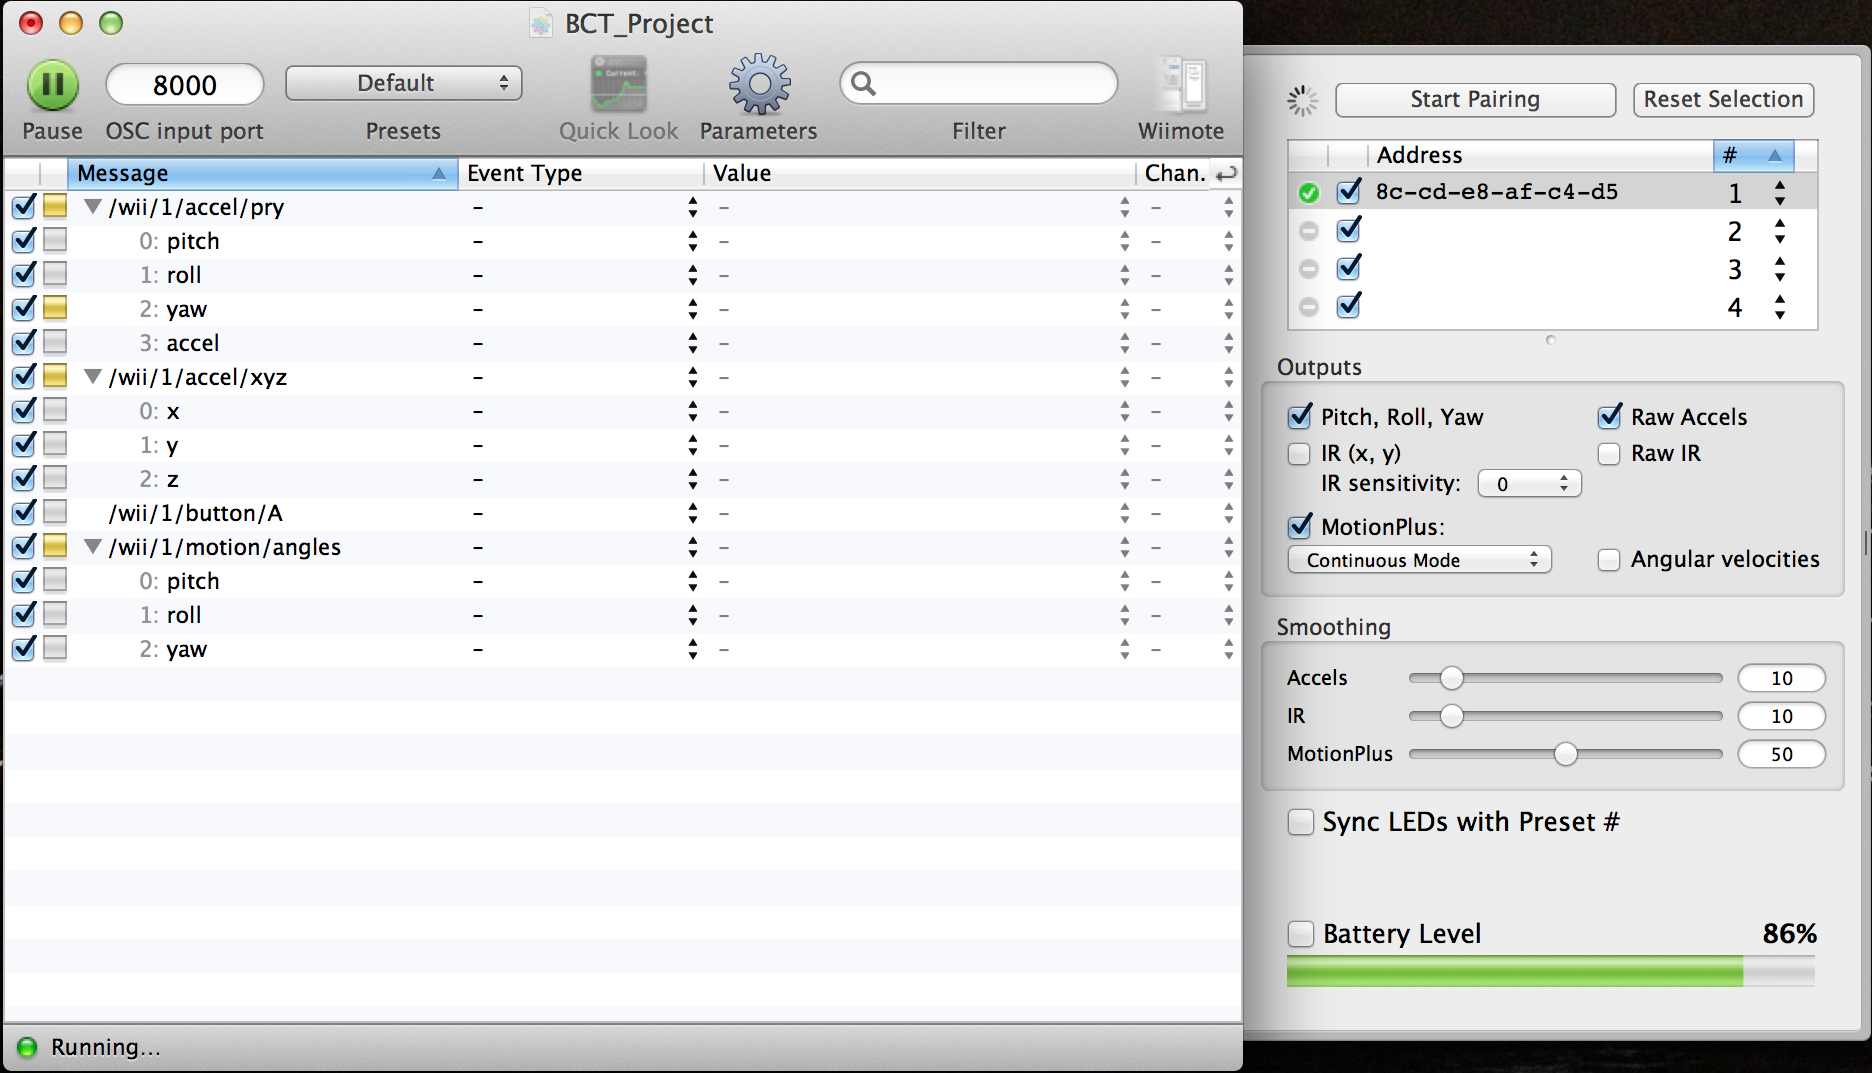
\includegraphics[height=0.4\textwidth]{osculator_1.png}
	\caption{OSCulator software receiving data from one Wii controller}

	\label{prototyping1.1}
\end{figure}

\begin{figure}
	\centering

	\subfloat[Wii controllers]{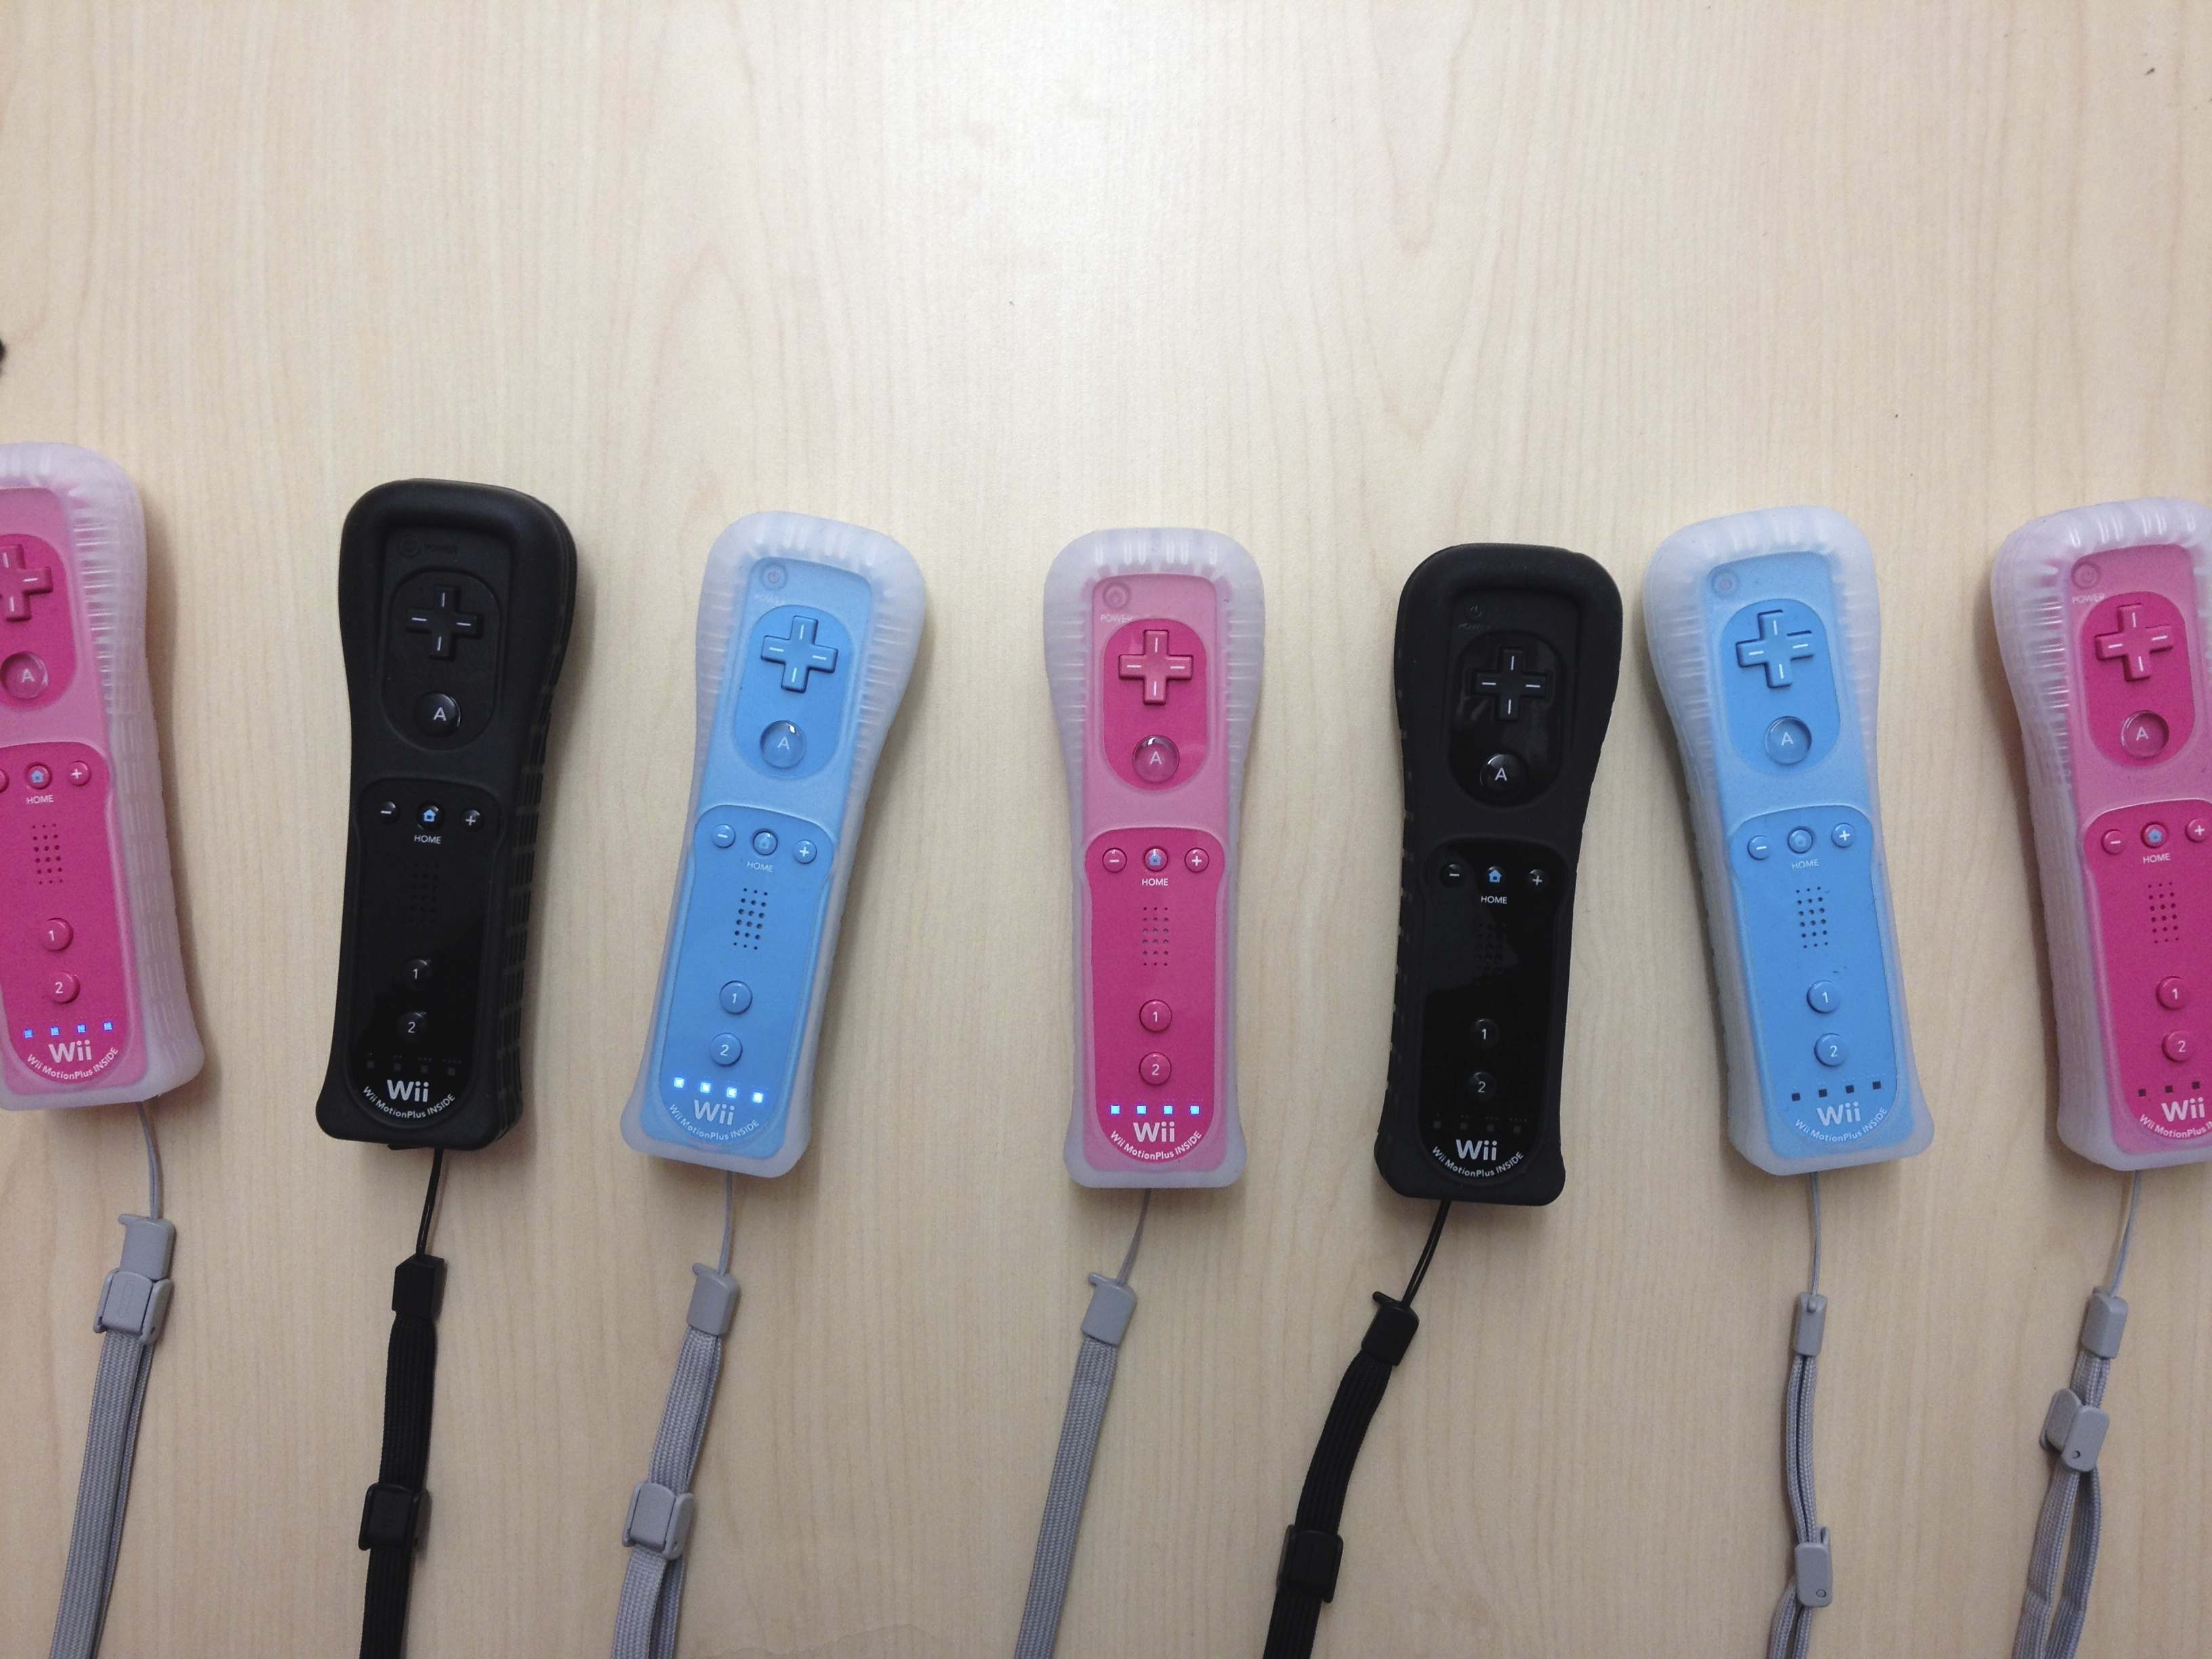
\includegraphics[height=0.32\textwidth]{wiimotes.jpg}}
	\hspace{0.1cm}
	\subfloat[Data successfully received from all controllers]{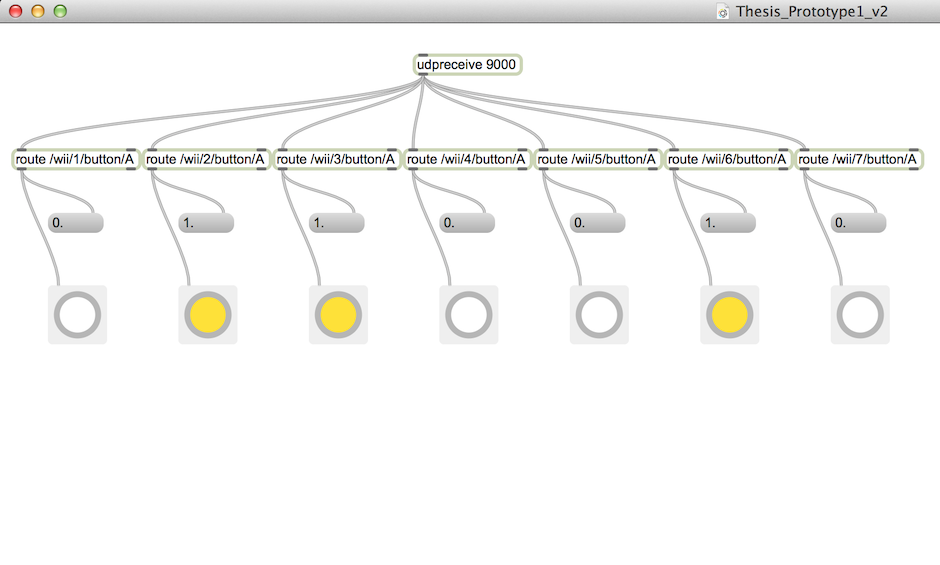
\includegraphics[height=0.32\textwidth]{multi_wii.png}}
	\caption{Testing simultaneous input from seven Wii controllers}

	\label{prototyping1.2}
\end{figure}

Upon syncing the Wii controller with OSCulator, I was immediately able to view movement and push-button data from my controller (see Figure \ref{prototyping1.1}). Next, I tested the limit of how many Wii controllers could connect to a computer. Since my thesis aims to give every member of an audience a new way to participate, this number would ideally be limitless. With Bluetooth technology, unfortunately, one master device (my computer) can only connect to a maximum of seven slave devices (Wii controllers). While a larger network could be established with some work, for the purposes of this prototype, I felt that seven controllers was sufficient. A Max patcher was created to display push-button data from multiple Wii controllers, and it worked as expected (see Figure \ref{prototyping1.2}).

My next task was to create the VJ system. After experimenting with a multitude of video effects objects in Max, I created a basic interface. The system is built around two short video loops that can be mixed together and modified. The user can crossfade between the two videos using the controller's Left and Right buttons. The resulting image can be rotated by rotating the controller sideways. A pixelation effect can be increased or decreased by increasing or decreasing the controller's incline. Finally, holding and releasing the A button enables and disables a motion blur effect. An important part of programming this patcher was mapping controller input to the effects controls. Values had to be carefully scaled and clipped in order for the user's movements to translate naturally to the effect they control. I also carefully selected the source video such that the effects of users' actions would be clear; a black and white clip of one person dancing and a colour clip of multiple people dancing seemed to offer adequate contrast.

With the details of the performance in place, the next step was selecting which aspect would be controlled by the audience. This was informed by Turino's (2008) concept of ``core" and ``elaboration" roles. In purely participatory performances, he explains, core participants are typically less skilled but work together to keep the performance going; elaboration roles, on the other hand, are reserved for experienced participants adding flourish to the performance. The audience, being the less-skilled party, would assume the core role. It was decided to give them control over the crossfader object -- a simple mechanism that can easily be controlled collectively. By pressing and holding the Left or Right buttons on their controllers, users could effectively vote on which video loop dominates the screen. In this case, for instance, if more people are holding the Left button than the Right, the black and white video would gradually become more prominent than the coloured video. Thus, while the audience collectively adjusts the tone of the visuals, the performer retains precise control over the other effects -- rotation, pixelation, and motion blur.

The last feature of this VJ system addresses a concern expressed by musicians in the ethnographic study -- giving the audience too much control.  In response to this, I provided the performing user with a `mute' function. By pressing their controller's B button, the performer can disable the audience members' controllers, moving control of the crossfader from the audience to the performer. This button is essentially an on/off switch for audience participation.

\begin{figure}
	\centering

	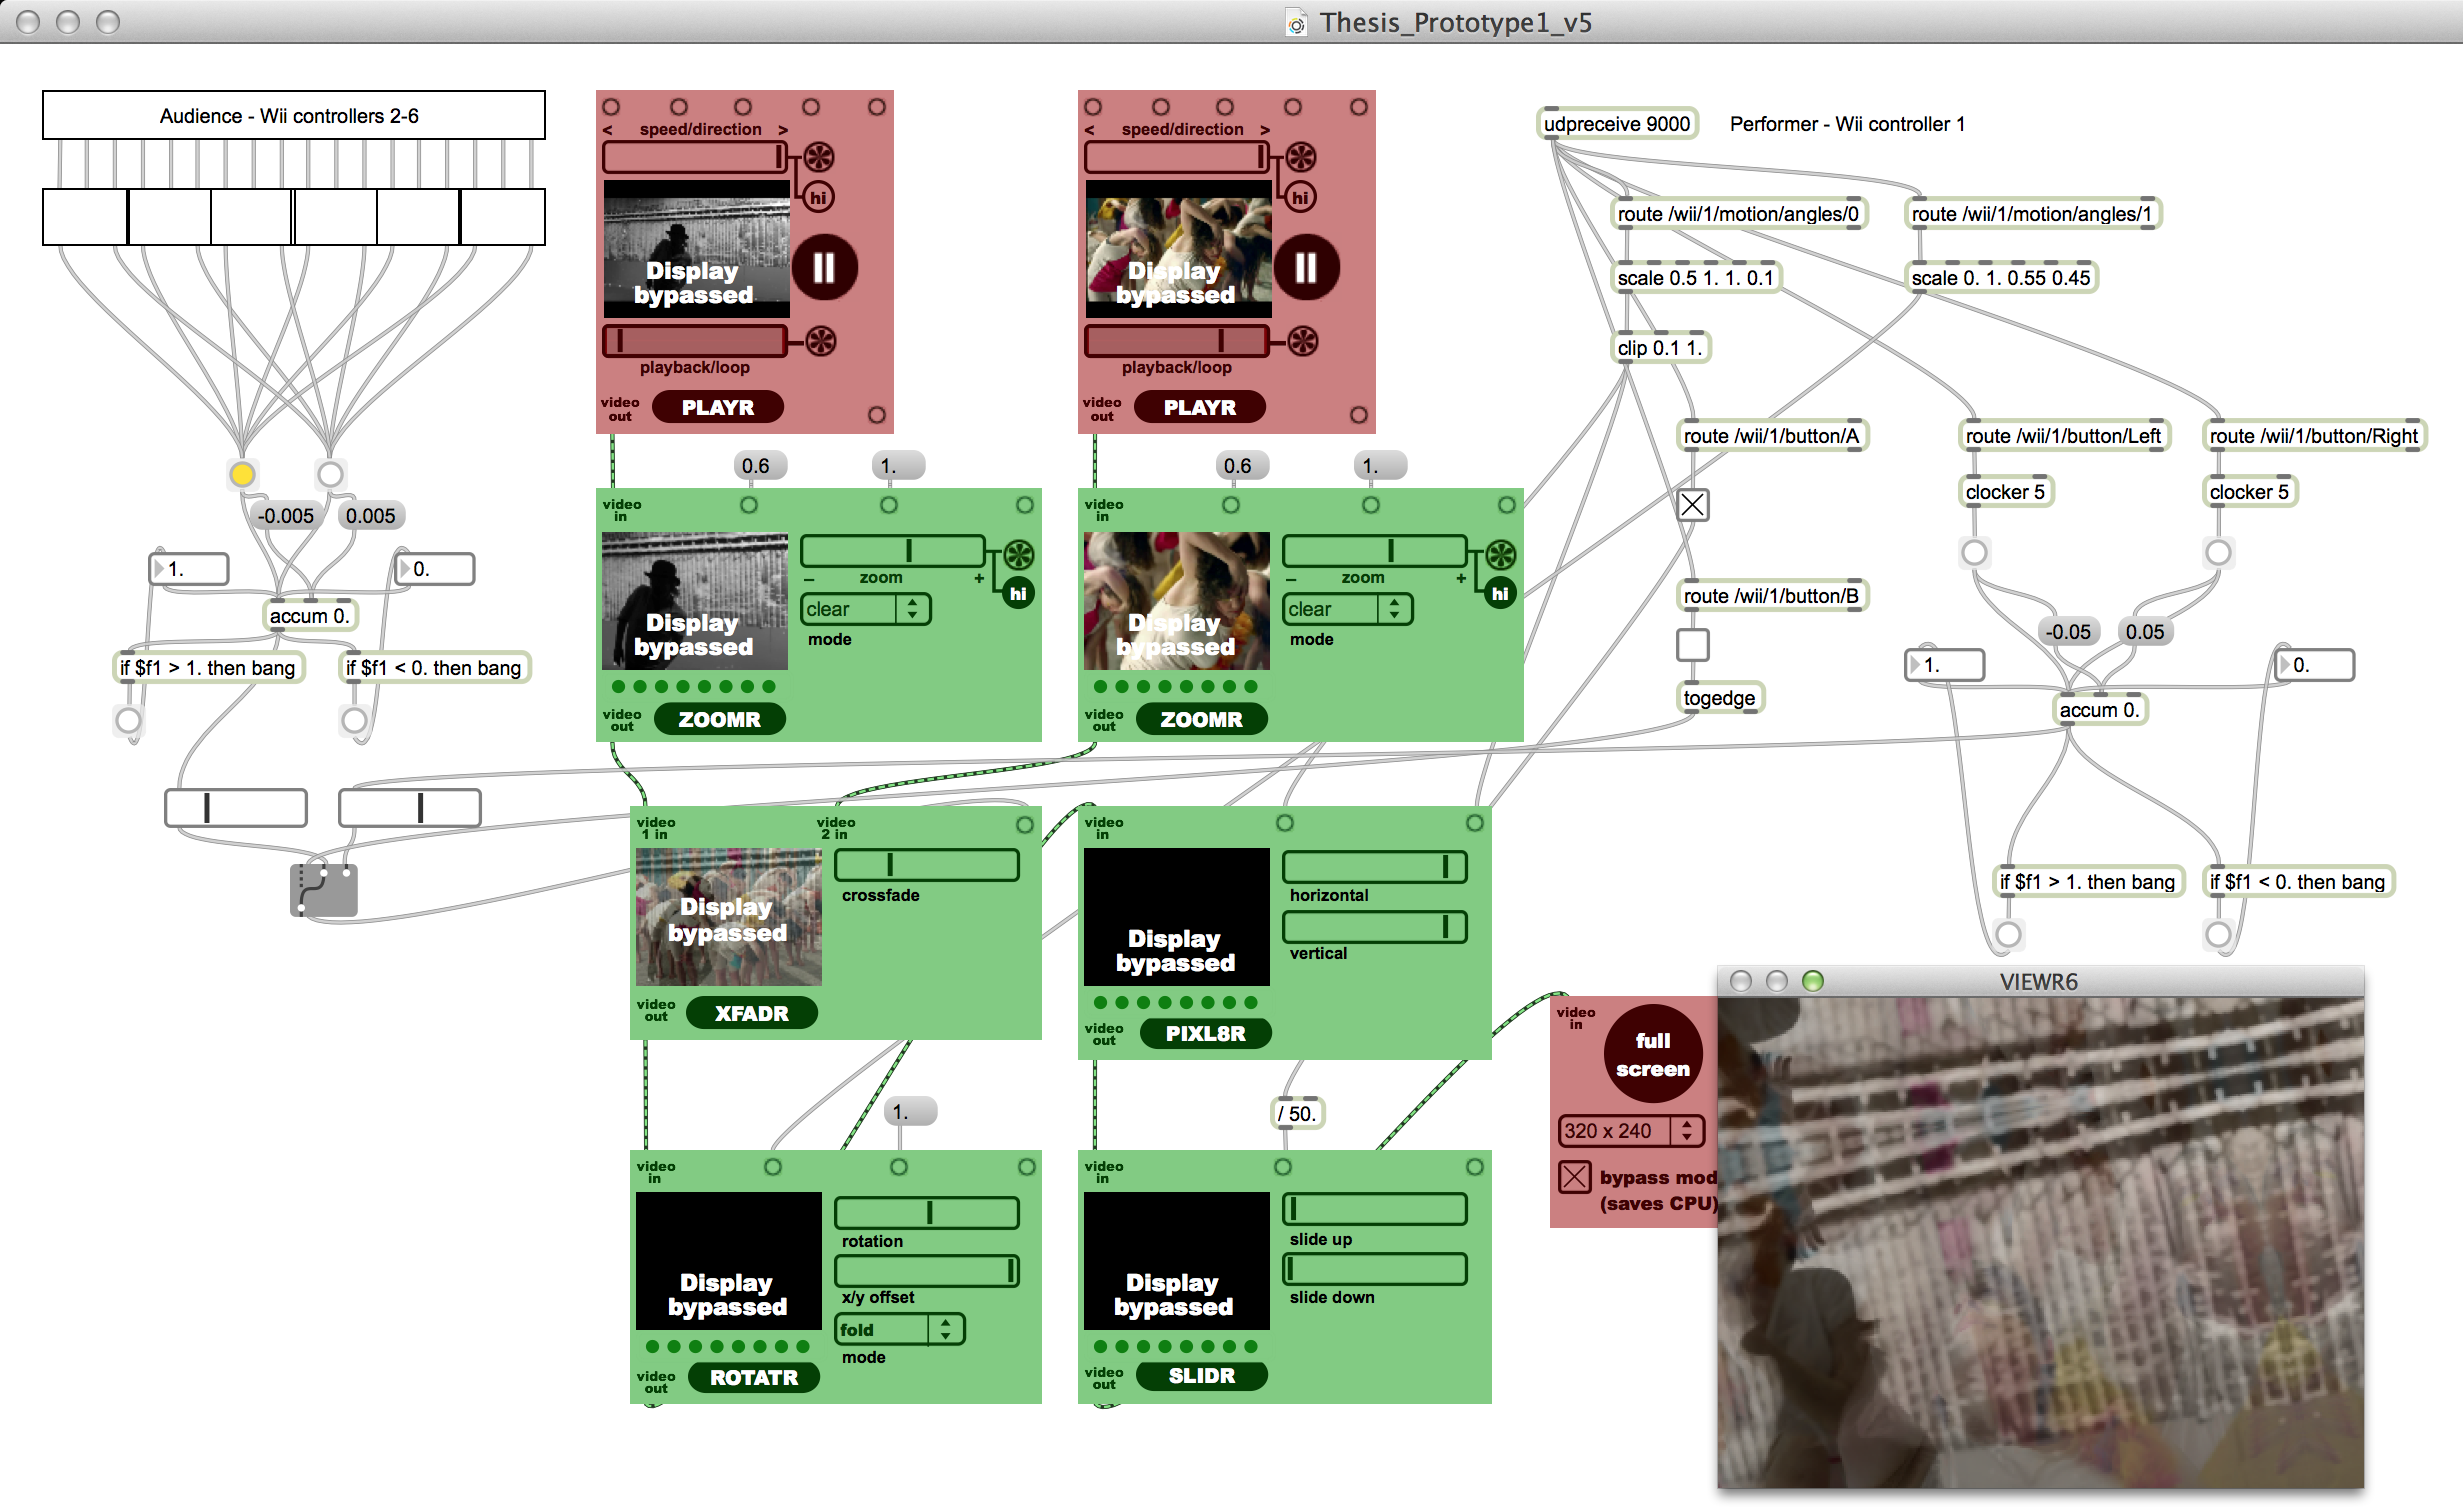
\includegraphics[height=0.4\textwidth]{vj_and_audience.png}
	\caption{Prototype \#1 Max patcher}

	\label{prototyping1.5}
\end{figure}

The completed patcher for the first prototype is shown in Figure \ref{prototyping1.5}.

\subsection{Testing}

The prototype's concept was presented at a research colloquium, and a group of attendees (students at OCAD University) participated in a brief demonstration. After illustrating the performer's controls, I invited participants to play with the collaborative crossfader mechanism. `Audience' users had no problems understanding the concept. As soon as users were given their controllers, one participant led the rest in first fading all the way to into one video clip and then all the way into the other. The system functioned as expected, and the group successfully made decisions and carried them out together. Finally, the performer's mute button was introduced, deactivating the participants' controllers to their amusement.

Some initial reactions were collected from colloquium attendees. First, it was suggested that there should be a focus on context; questions would best be answered in a real live music setting. It was asked if this sort of system should be goal oriented; if not, would the users somehow turn it into a game anyways? Several people agreed that some form of direct feedback should be provided to users. One attendee wondered if every audience member could be individually represented, rather than treating the group as a single unit. Discussion led to talking about `the wave' -- where individual participants perform a simple action to create a large, impressive visual effect. It was also asked how my system would react if some audience members did not wish to participate.

\subsection{Analysis}

The willingness of users to participate and the amount of discussion that was sparked confirmed that this research is of interest to the public. This prototype raised many points to be considered for future iterations. For example, it was encouraging to see the users immediately begin collaborating. Facilitating this tendency could make future iterations more intuitive for users. The voting system implemented in this prototype, however, is likely not the best way to promote collaboration. This left-versus-right model could easily create a competitive, goal-oriented environment instead of a performative one. The voting system's many-to-one mapping also presents problems with feedback; the results of each user's actions are combined and thereby obscured. How can future prototypes provide clear, individual feedback while still effectively contributing to the overall performance? Furthermore, how can a system react if only a portion of an audience chooses to participate? One feature that raised no issues was the mute button; it seems sensible that future work should continue allowing performers to regulate audience control.

Further reflection led me to contemplate the nature of the participation. This prototype involved the audience directly influencing a performer's primary creative output -- similar to D'CuCKOO's MidiBall or Freeman's (2005) \textit{Glimmer} project. Projects like PixMob or Xylobands, however, are different: while the performance's primary output is live music, the audience is only participating in the light show -- what I am calling the secondary output. As emphasized by the ethnographic study, and as is reasonable to assume, the average performer is hesitant about allowing others to influence their primary output. Thus, a participatory technology would likely be more desirable to performers if it was limited to secondary output.
% Move this to Prototype #3 Analysis?
% Audience survey indicated an equally low interest in influencing both the music and the lights

% Prototype #1 Outcomes:
% * People are interested in participating in performances
% * Collaboration happened naturally
% * Decision based inputs could create a goal-oriented environment instead of a creative one
% * Many-to-one mapping sucks for feedback
% * A mute button is useful -- regulated audience input
% * A participatory system should probably only influence secondary output in a rock concert setting

\section{Prototype \#2}

% Motivation:
This prototype's purpose was to explore possible input mechanisms for audience members. Through user testing, I hoped to identify which were intuitive, which were most natural and meaningful to perform as a group, and which afforded accurate collaborative control.   This prototype also allowed for exploration of different feedback methods. Lastly, by basing it around the voting-based VJ system from Prototype \#1, I hoped to make conclusions about goal-oriented systems and the crowd behaviours that result from them. After receiving the opportunity to participate in the eLeo exhibition at OCAD University, it was decided to design this prototype as an interactive installation. By inviting the exhibition attendees to test the various methods of input, I could observe their behaviours and collect reactions from a wide variety of users.

% Prototype #2 Goals:
% * Find what types of audience actions are effective input mechanisms
% * Start investigating feedback solutions

\subsection{Development}

From the start, it was clear that body movement would be a more fitting input than something like button pressing. Most users find movement-based interactions satisfying (Ulyate \& Biancardi, 2001); plus, there are apparent subconscious ties that link music and movement (Jourdain, 1997; Levitin, 2006), making this a natural form of input for a live music environment. In designing their audience-interaction system, Barkhuus and J{\o}rgensen (2008) found that motions based on already-present behaviour were especially effective input methods. I created a list of common crowd behaviours to be incorporated in the prototype -- giving a thumbs up or thumbs down, swaying one's arms back and forth, clapping, and doing `the wave' (also known as `the Mexican wave').
% Survey participants indicated that they regularly move in various ways at shows
% Researchers emphasize the importance of meaningful feedback in crowd-controlled systems (Ulyate \& Biancardi, 2001; Barkhuus \& J{\o}rgensen, 2008), and this was also a recurring concern in the response to Prototype \#1.

\begin{figure}
	\centering

	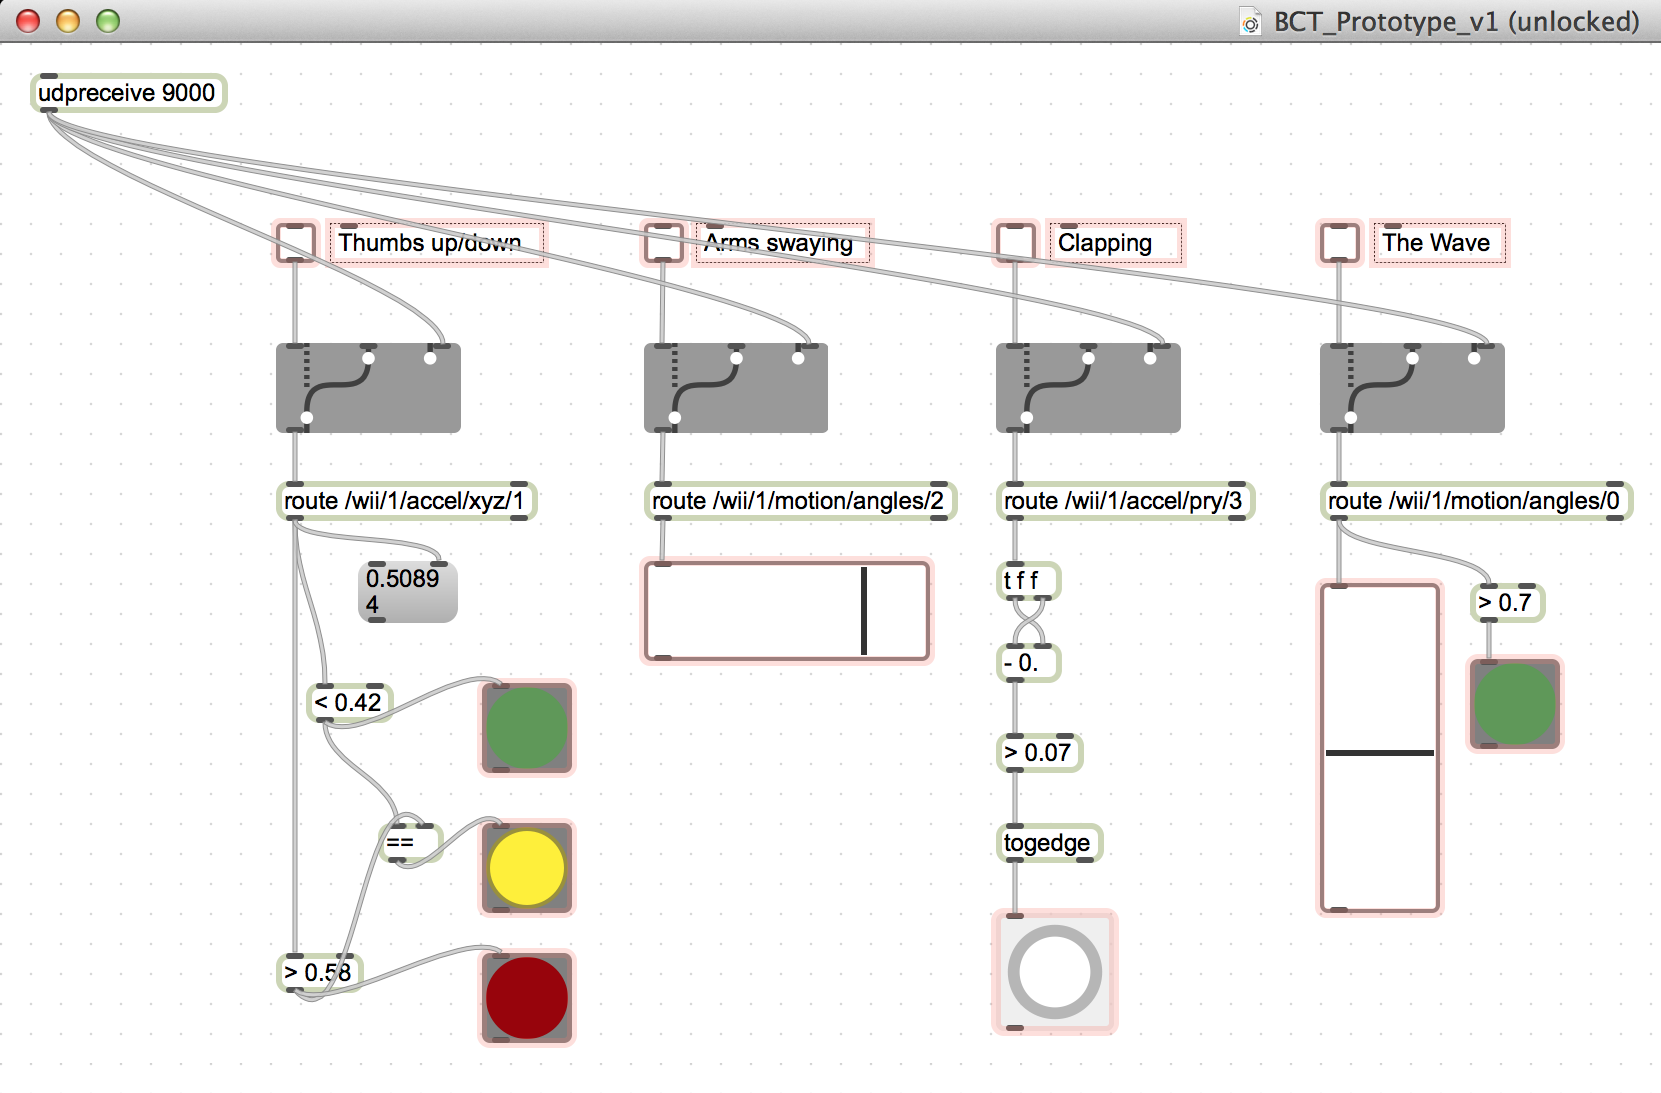
\includegraphics[height=0.4\textwidth]{wiimote_audience.png}
	\caption{Monitoring thumbs up/down, arm swaying, clapping, and the wave}

	\label{prototyping2.1}
\end{figure}

The first prototype provided a suitable framework for this experiment: I continued using multiple Wii controllers as input devices, and OSCulator was used to route the data to Max where it processed and represented visually. From here, I needed to be able to recognize when a user was performing one of the selected crowd behaviours. By pulling data from the controller's motion sensors, I was able to identify when the user was giving a thumbs up or down, swaying their arms left or right, clapping, or doing the wave. I incorporated simple visual feedback -- LED objects that light up when the user points their thumb up or down or claps, and sliders that follow arm movement when the user is swaying or doing the wave. Calibrating these required trial and error tests using different thresholds -- determining what amount of acceleration qualified as a clap, for instance. Figure \ref{prototyping2.1} shows the first iteration of this prototype.

\begin{figure}[p]			% On its own page
	\centering

	\subfloat[Thumbs up/down]{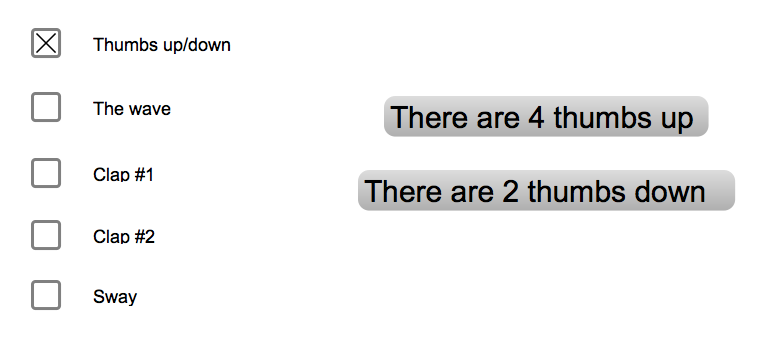
\includegraphics[height=0.2\textwidth]{thumbs.png}}
	\hspace{0.1cm}
	\subfloat[The wave]{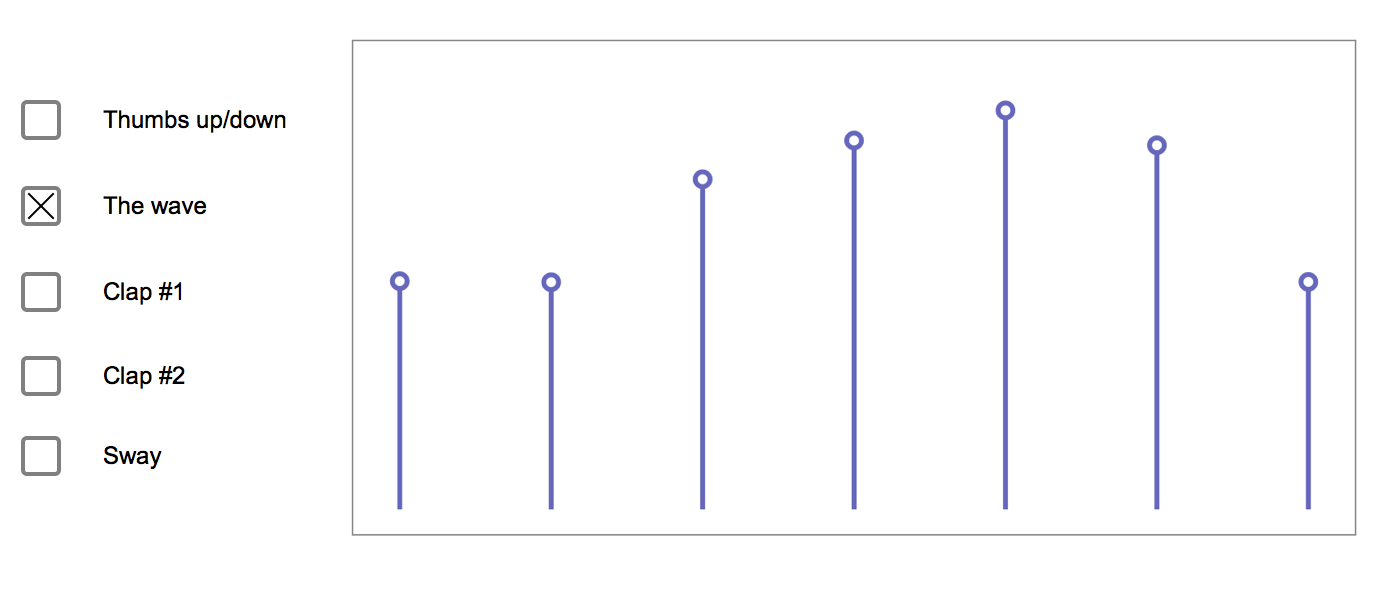
\includegraphics[height=0.2\textwidth]{wave.png}}	
	\hspace{0.1cm}
	\subfloat[Clapping]{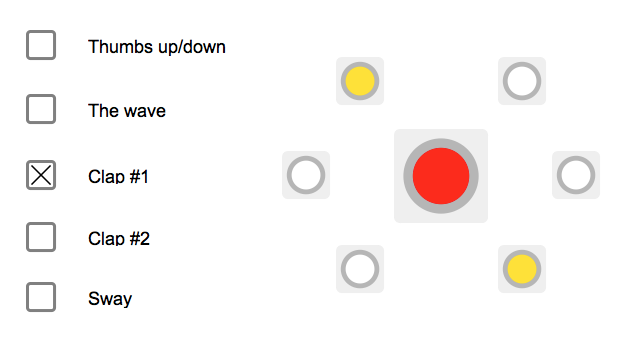
\includegraphics[height=0.2\textwidth]{clap1.png}}
	\hspace{0.1cm}
	\subfloat[Clap-o-meter]{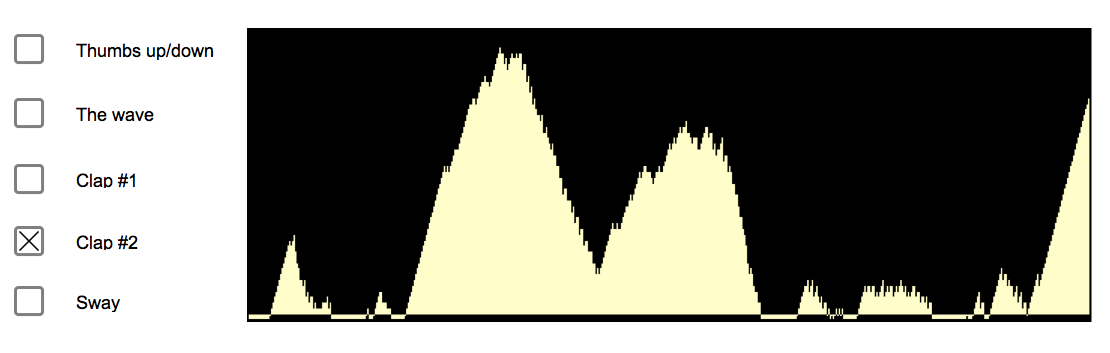
\includegraphics[height=0.2\textwidth]{clap2.png}}
	\hspace{0.1cm}
	\subfloat[Arm swaying]{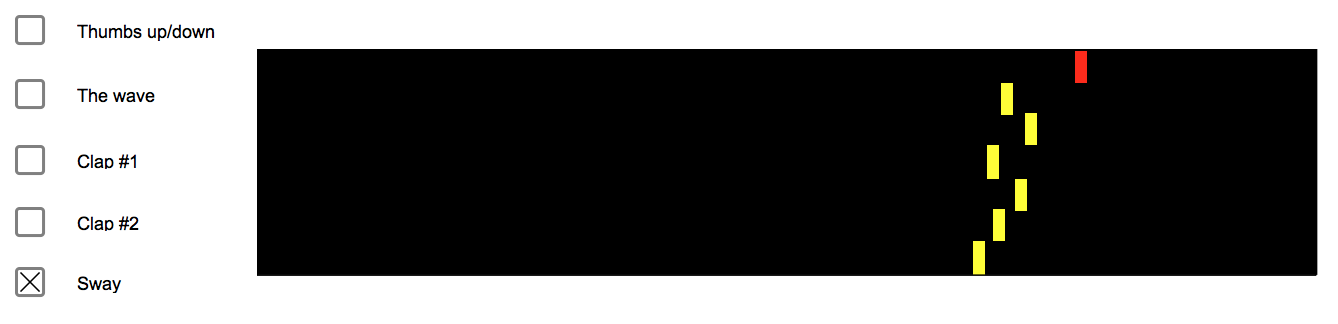
\includegraphics[height=0.2\textwidth]{sway.png}}

	\caption{Input methods}

	\label{prototyping2.2}
\end{figure}

Next, I modularized the patcher and multiplied it sevenfold. The actions of seven users could now be monitored simultaneously. I developed new visualizations to reflect these multiple inputs, shown in Figure \ref{prototyping2.2}. Thumbs up/down mode simply displays how many users are holding their thumbs up and down. The wave mode shows the vertical position of each user's arms. I created two modes to detect clapping. The first displays seven LED objects that illuminate when each user claps, encouraging users to clap in sync. The second mode -- a `clap-o-meter' --  was included to compare how users react to collective visualizations compared to the other modes' individual representation.  Lastly, the swaying mode includes a slider to display the left-right movement of each user.

Two additional modes were added at this point to act as controls. The first invites users to imitate holding a lighter in the air. This is done by holding the Wii controller upright and pressing the A button, causing LED objects on the screen to illuminate. I included this button-based input to observed how user response compared to that of a motion-based input. In the final mode, users are simply invited to dance. The visuals displayed on screen are generated randomly; the users are not actually controlling anything. This was included to see how users responded when the effect of their actions was completely unclear.

\begin{figure}
	\centering

	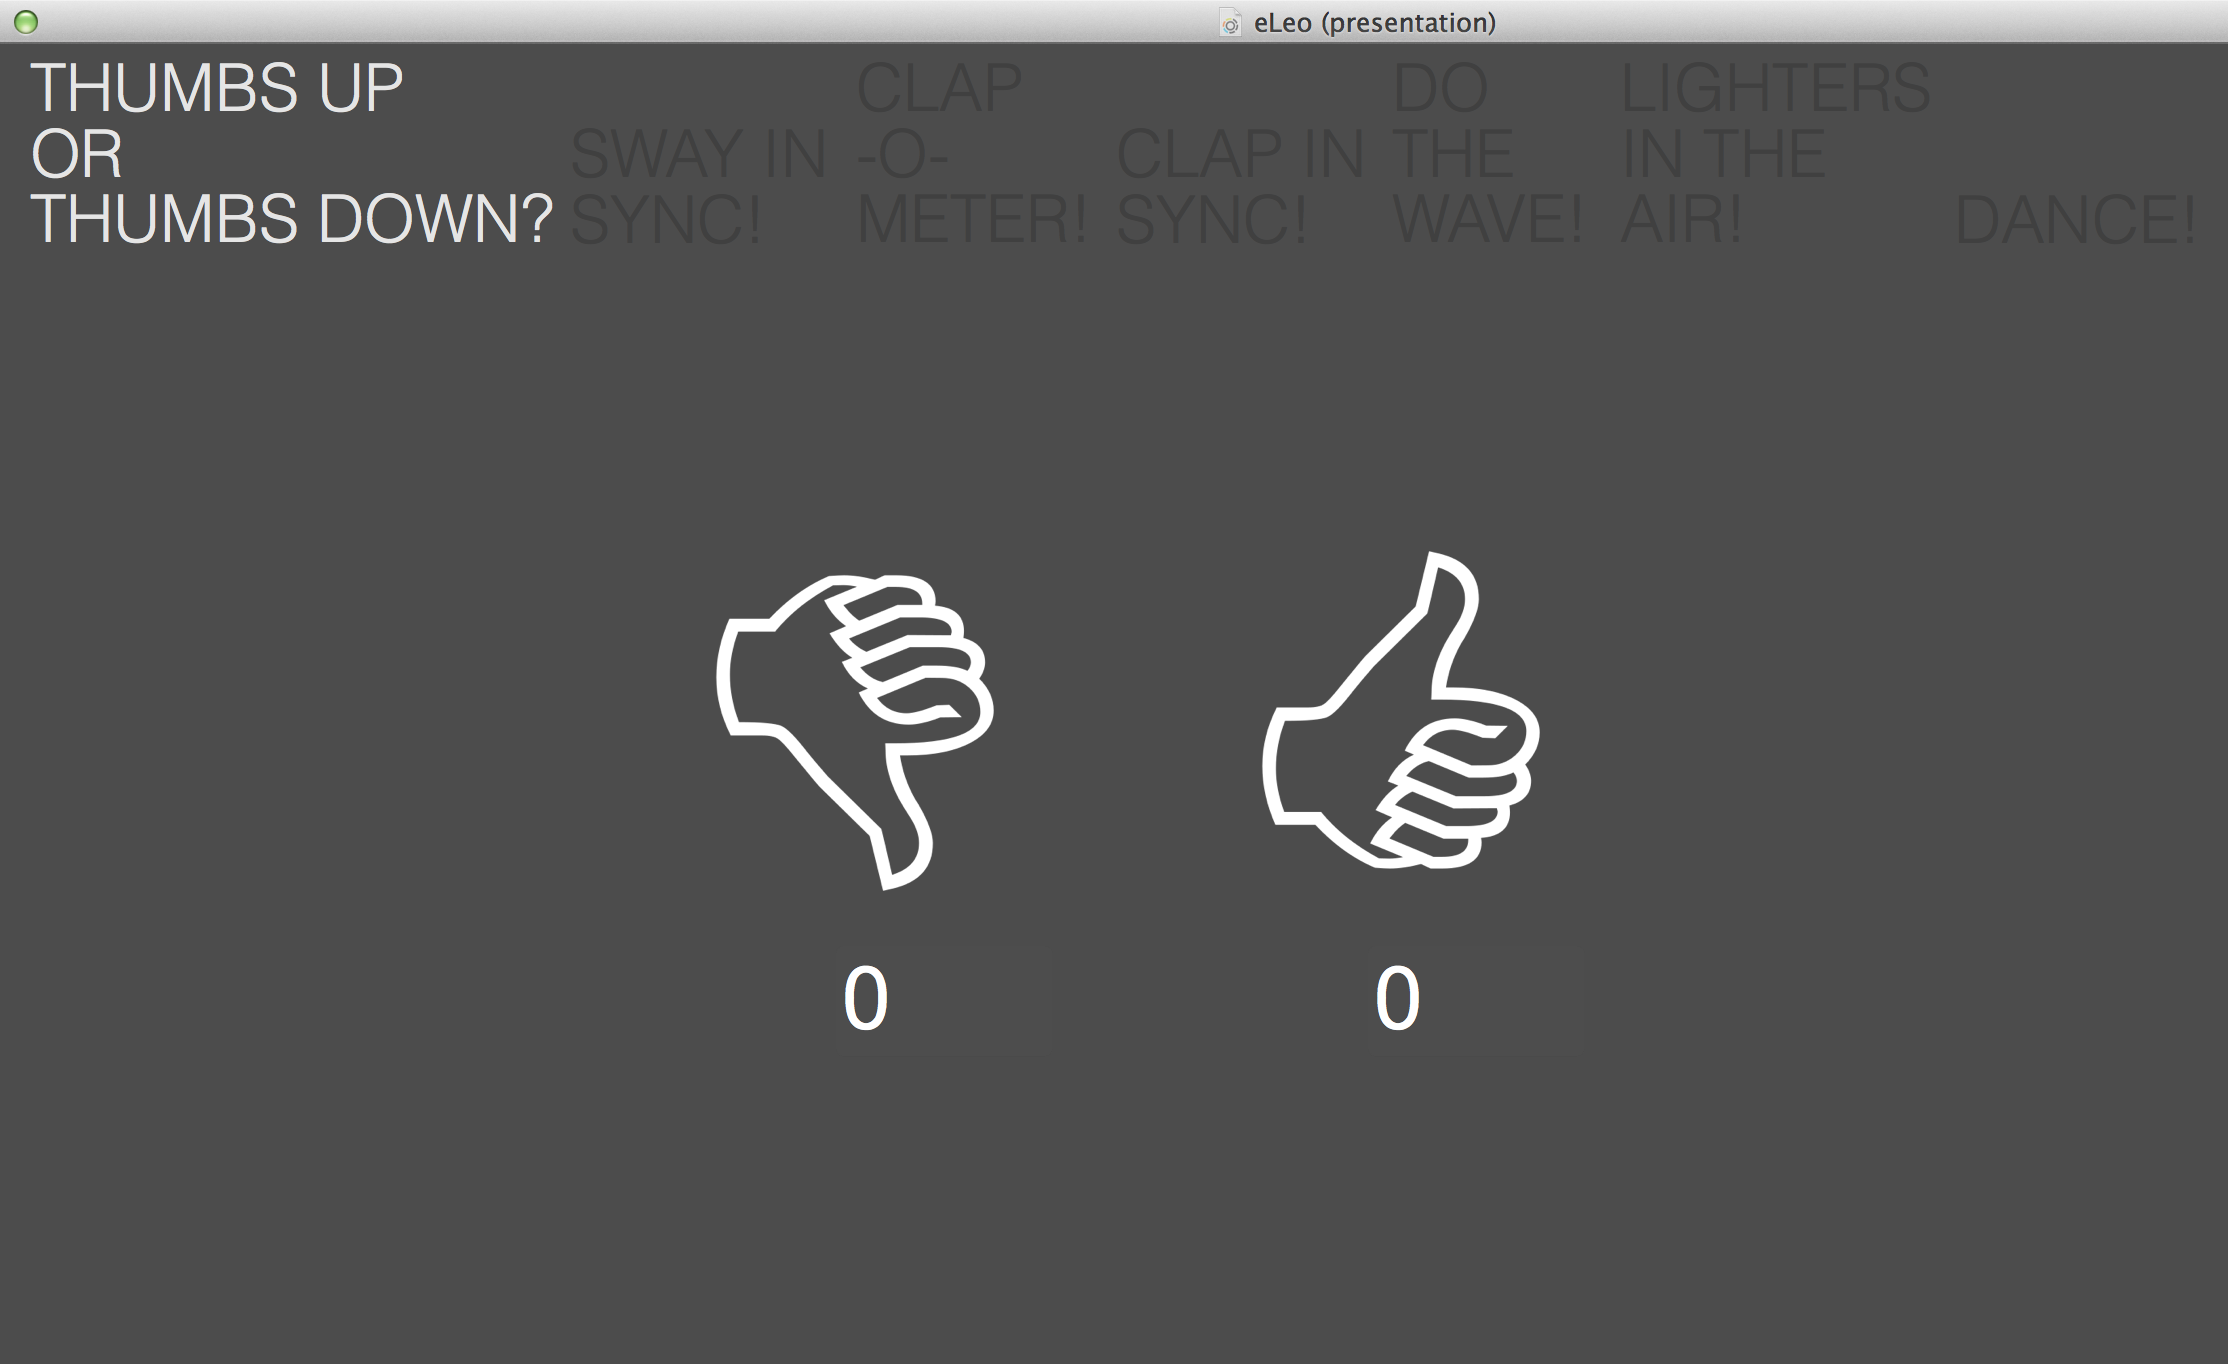
\includegraphics[height=0.4\textwidth]{presentation.png}
	\caption{Input prompts}

	\label{prototyping2.3}
\end{figure}

In preparation for the exhibition, I modified the patcher to function as an installation. An auto-play function was implemented; the input methods are looped through automatically, each activated for ten seconds at a time. A short text prompt is displayed to give users a hint at what action they should be performing (``Thumbs up or thumbs down?" ``Sway in sync!" ``Clap-o-meter!" ``Clap in sync!" ``Do the wave!" ``Lighters in the air!" ``Dance!") as shown in Figure \ref{prototyping2.3}. Thus, the system would not require an operator, and users could approach it at any time during the exhibition and test each mechanism.

Lastly, part of the VJ system from Prototype \#1 was added to the patcher. Namely, the crossfade system was implemented and connected to each input mechanism. For instance, in swaying mode, if all users swayed their arms to the left, the slider would move to the left and the black and white video loop would overtake the colour loop. In clap-in-sync mode, the colour video would play only if users manage to consistently clap together.

\subsection{Testing}

\begin{figure}
	\centering

	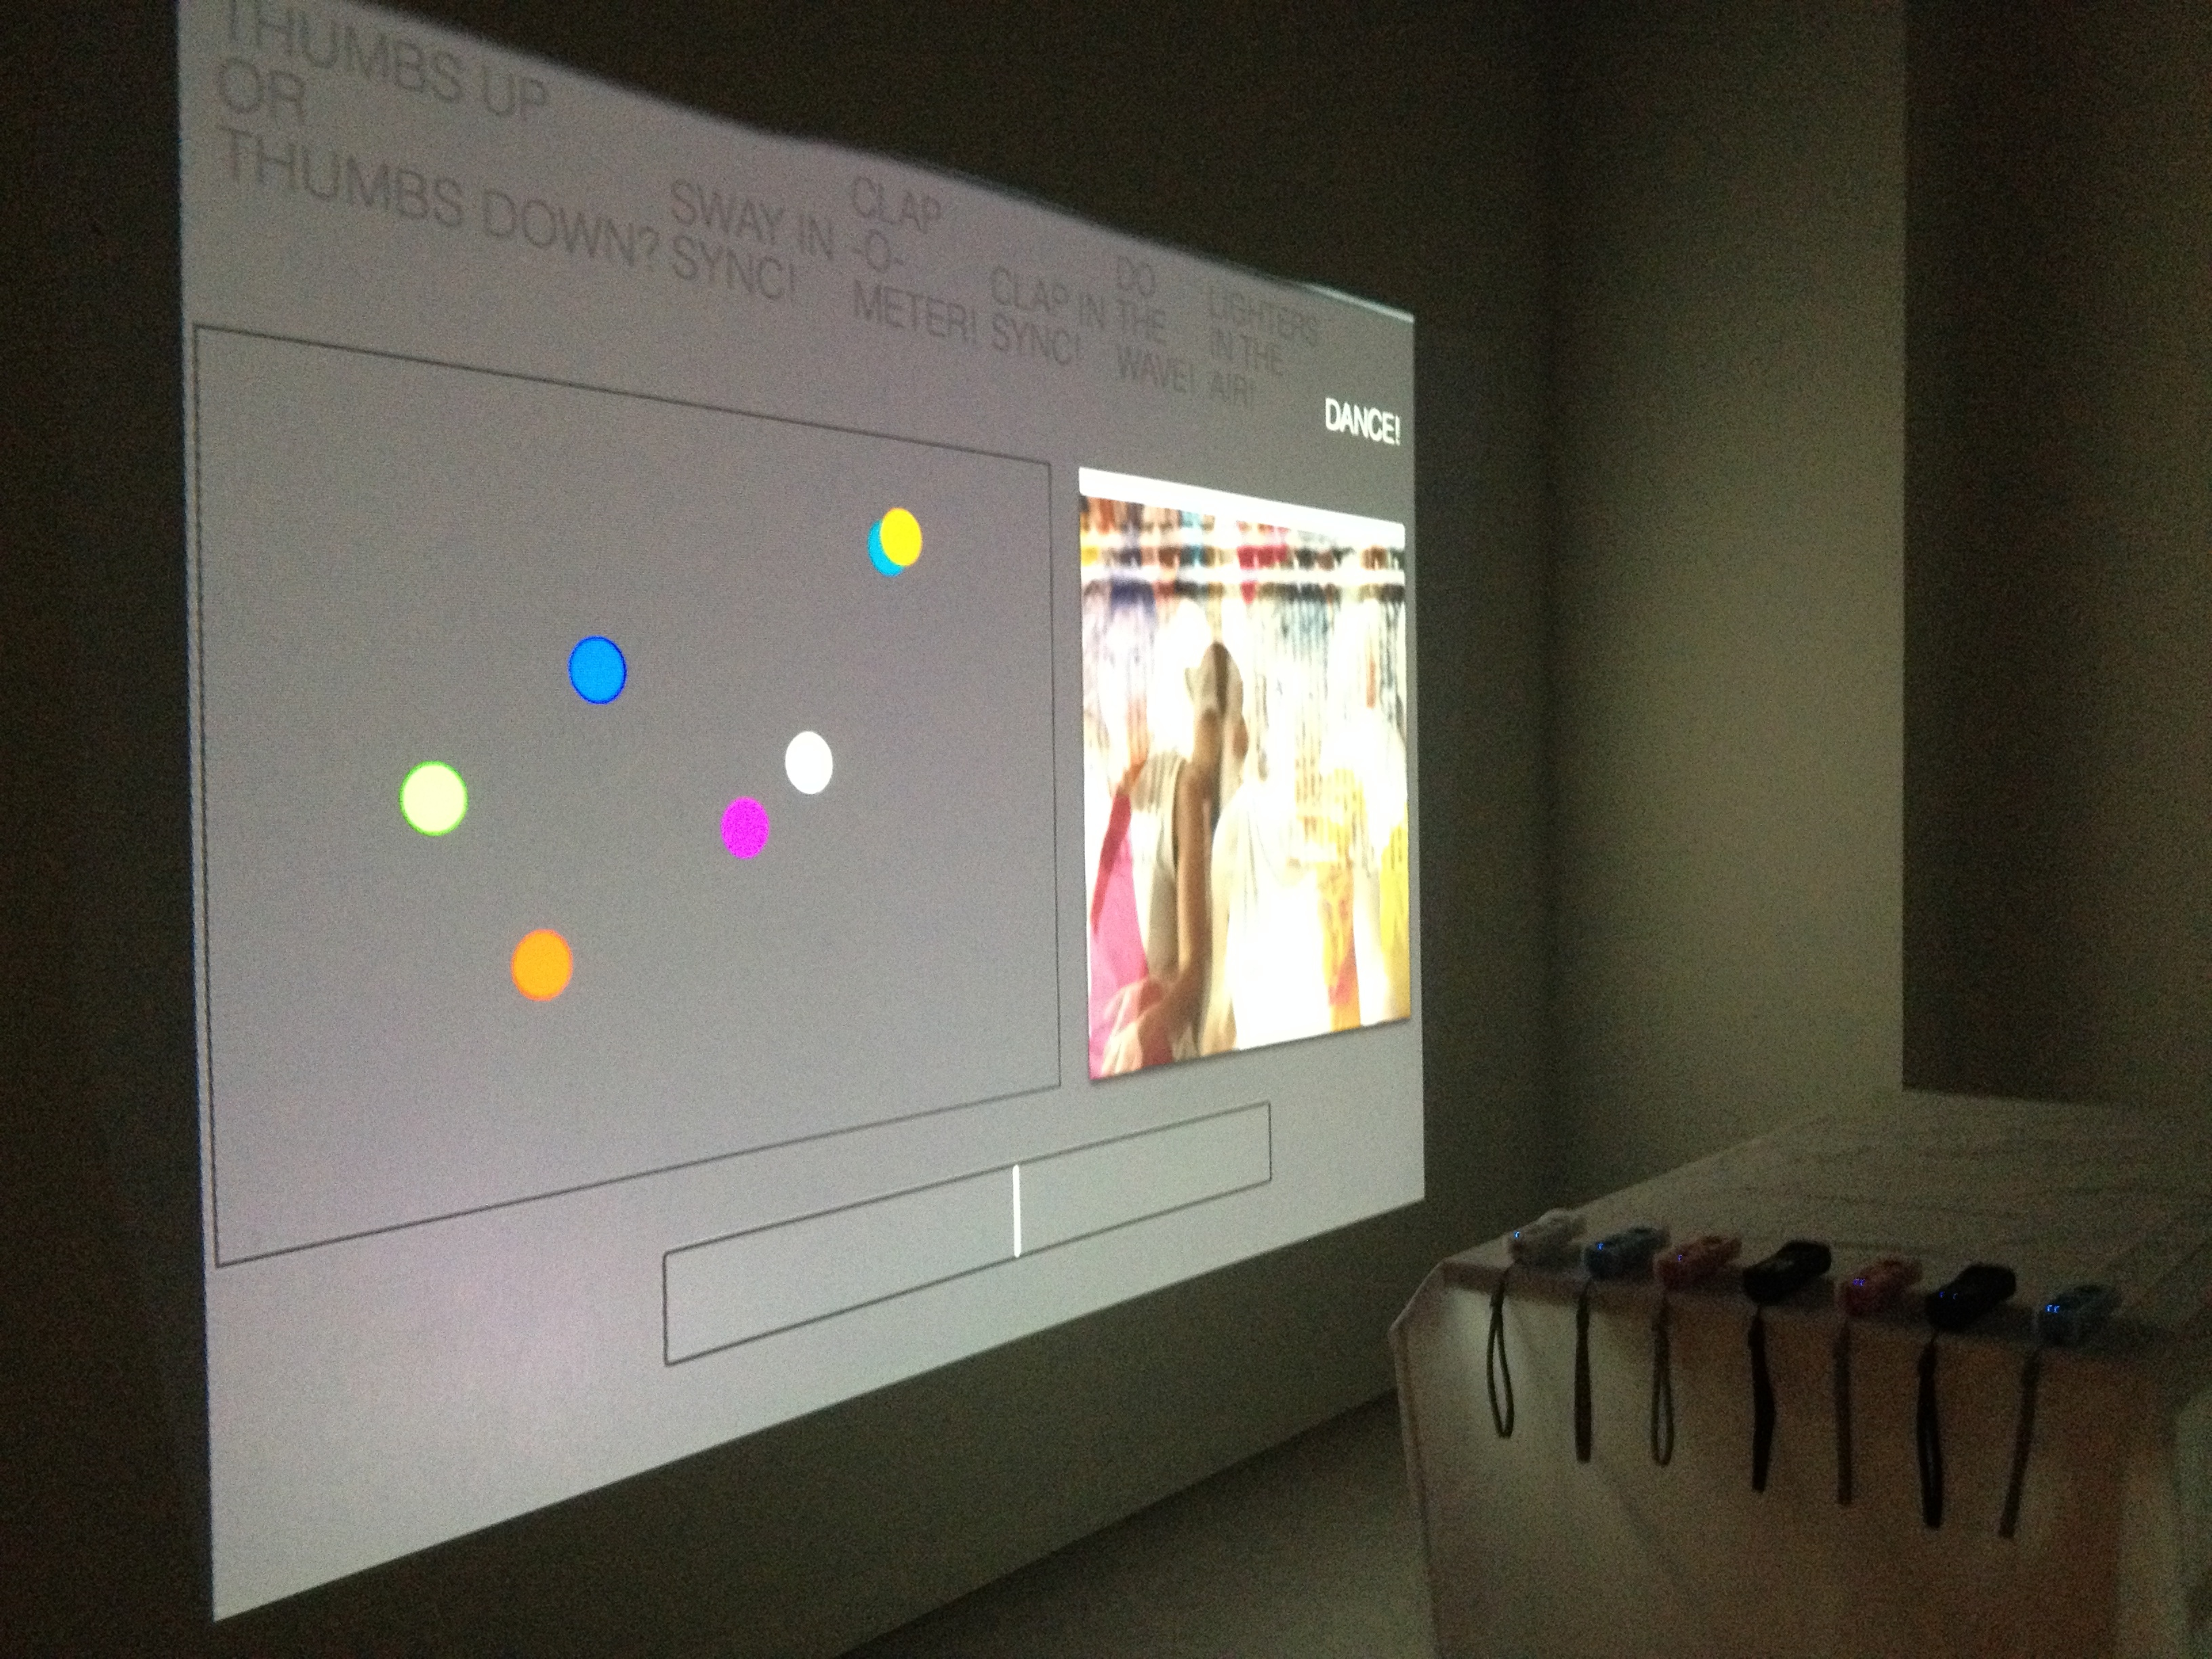
\includegraphics[height=0.4\textwidth]{eleo_1.jpg}
	\caption{Prototype \# 2 installed at the exhibition}

	\label{prototyping2.4}
\end{figure}

Testing took place over a few hours during the opening night of the eLeo exhibition at OCAD University. The final patcher was projected on a large wall in a darkened room using a short-throw projector. The seven Wii controllers were laid on a table in the middle of the room, their LEDs illuminated, inviting users to pick them up. Figure \ref{prototyping2.4} shows the prototype set up in the exhibition. Approximately twenty users engaged in the installation for extended amounts of time.

Given the casual nature of the event, attendees were relaxed and generally openminded. Groups that entered the room were asked if they were interested in participating in an experiment. Those that accepted were briefed in one of two ways. Half of the groups were told the experiment's motivation -- that I was investigating how audience behaviours could be turned into inputs at live music events. The other half were given no information. I did this to see how users would approach the system with minimum instruction. Indeed, some of those who received no information were unsure of what was expected of them. Some only pressed buttons on their Wii controller, sometimes holding it in front of them and pointing it at the screen. One user wondered aloud what their goal was.

Those who were given context understood the system much more easily, quickly figuring out that they could perform physical motions as a group and manipulate the video. Some users invited bystanders to grab a controller and join them, eager to test the system's capabilities. Each input mechanism received different reactions. As I observed and spoke with participants, some general opinions of each method began to surface.

\subsubsection{Thumbs Up or Down}
Most users understood this action quickly. Some tilted the controller left and right, not fully inverting it for a thumbs-down input. Others simply started shaking the controller. The up-versus-down counter seemed random to many users at first. As groups started to understand the system, they coordinated inputs -- all thumbs up or all thumbs down. Users commented that the thumbs-down motion was difficult to perform. Some commented that the up/down action seemed strange to link to the left/right movement of the crossfader slider.

\subsubsection{Sway in Sync}
Users had trouble identifying which slider was connected to their controller. Some solved this by shaking the controller violently and observing which onscreen slider was moving accordingly. Some users were holding the controller backwards, causing their input to be reversed and adding confusion. All groups eventually organized themselves and began swaying in sync. Most users did not raise their arms in the air, instead casually hold the controller in front of them; in conversation, they indicated that they did not feel compelled to lift their arms since the visuals responded regardless.

\subsubsection{Clap-O-Meter}
Since this visualization reacted gradually, users were initially confused, and several commented on the slow response. While some said that the visualization was appealing, many agreed that they would preferring seeing individual outputs. Some groups worked together and tried to fill up the clap-o-meter. Some users expressed uncertainty about clapping with the controller in their hand, complaining that it was painful to hit it against their palm. Overall, users seemed to tire of this mode quickly.

\subsubsection{Clap in Sync}
All users quickly caught on to this mode. In most groups, one participant would lead the others by counting out a time. Users commented that it was a fun challenge to try to clap in sync. However, once synchronization was achieved for a few seconds, most groups felt they had completed what was expected and stopped. Some users also commented that the minor lag in the visualization was distracting.

\begin{figure}
	\centering

	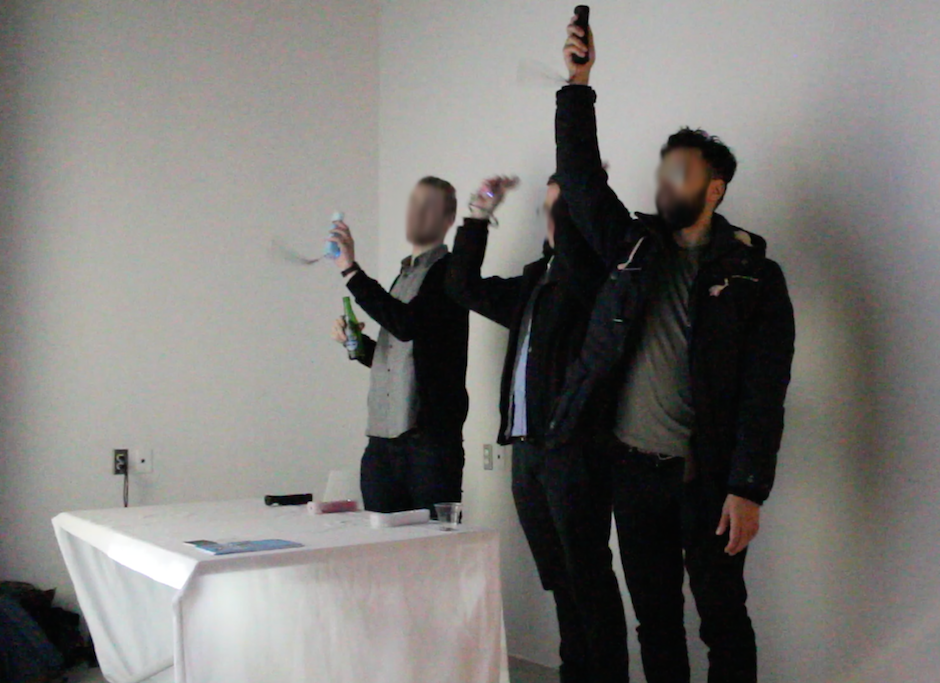
\includegraphics[height=0.4\textwidth]{testing.png}
	\caption{Three users experiment with Prototype \#2}

	\label{prototyping2.5}
\end{figure}

\subsubsection{The Wave}
Nearly all users instantly understood this prompt and were eager to raise their arms in the air. Figure \ref{prototyping2.5} shows three participants performing the wave input. While one group did not communicate and focused on their own slider, most cooperated to raise their arms simultaneously. One group even organized themselves in a row such that they were in the same order as their corresponding onscreen sliders. Users enjoyed the appearance of this visualization. Although, a particularly thought-provoking comment was made by one user: this electronic representation of the wave was less satisfying than watching the wave itself.

\subsubsection{Lighters}
Most users instantly understood this input as well. A few tried to see if pushing the button rapidly would create a different response. Some groups worked together to light up all the LED objects together. This mode seemed unexciting to most users; one vocalized her boredom.

\subsubsection{Dance}
Many users responded to this prompt without hesitation and began moving. Others were clearly not comfortable doing so. Groups expressed confusion over the random visualizations and tried to make sense of their role. When told their input had no effect, some users were slightly annoyed.\\

\noindent
In multiple modes, users noted that they were not paying attention to the video loops and were rather focusing their attention on their corresponding sliders and LED objects. One user suggested that if the system were incorporated into a live performance, the clips could be replaced by two live video feeds of the performance itself.

\subsection{Analysis}

Several revelations came out of this prototype regarding input mechanisms. Inputs based on already-present behaviour were generally intuitive for users. The Wii controllers raised some issues, however; buttons distracted some users, and inputs could not be successfully performed when the device was held in unexpected orientations. Measures should be taken for future prototypes to avoid or adapt to such incorrect use. As the first prototype began to show, modes that rewarded collaboration here received the most immediate responses. However, when users felt that there was a goal, they stopped participating once they believed that it was achieved. The text prompts that were used in this system seemed to place limits on the users and should be excluded in real-world participatory systems.

Testing also provided insight on feedback methods. Individual visualizations for each user, such as the clap-in-sync LEDs or the wave sliders, were most effective. This was reinforced by the fact that most participants did not pay attention to the video output; users wanted to look at their individual influence on the system more than the collective results. Immediate feedback is also crucial; unlike the clap-o-meter, a system should allow users to quickly discover how they can influence it. Lastly, it is important that watching the overall output is more captivating than watching others perform the input itself.

% Prototype #2 Outcomes:
% * The buttons were misleading
% * Preference for individual visualizations for each user (i.e. not Thumbs up/down or Clap-o-meter)
% * On/off is most appealing. Choosing between two options caused confusion (i.e. no more left/right voting). This is just like regular audience behavior I guess?
% * Collaboration came naturally and was enjoyable. Many users counted time.
% * Direct control of visual elements trumps indirect control (i.e. ditch the video crossfading)
% * Users should be able to opt out without affecting others' experiences (i.e. not Thumbs up/down or Clap-o-meter)
% * No forced goals (i.e. no prompts to perform in sync). Allow for creativity.
% * Be clear about the rules of the system or users will begin experimenting and become distracted
% * The output must be more captivating than the input (i.e. no digital wave)


\section{Prototype \#3}

The final prototype took the form of a collaboration with one of the ethnography subjects, Toronto musician Christian Hansen. After our interview, he expressed interest in incorporating one of my prototypes into a performance. My ethnographic study made it clear that each performer has a unique opinion on what makes a great performance; thus, I knew that it would be important to develop a new prototype in close collaboration with Christian and ensure that the system reflected his performance style.

% Description of the band:
The current incarnation of the Christian Hansen band features Christian providing lead vocals and Molly playing keyboard, performing backup vocals, controlling backing tracks, and shaking a tambourine. Both bring high energies to their performances; Christian frequently moves around the stage, dances, and sings very expressively, and Molly, despite being stationed behind a keyboard, continuously moves to the music as well. The band does not typically use any more equipment than is needed. They aim to make a big impact through simplicity and rawness. As explained in Chapter 4, Christian often involves the audience in performances, encouraging singalongs and moving between the stage and the crowd. He feels that it is his job to maximize the audience's energy level.

% The band's desires:
The band expressed interest in allowing the audience to control their light show in some way. Christian wanted a system that could unite audience members without turning into a distraction from the music. He also expressed concern about giving the audience too much control; only the band should be able to dictate the flow of the performance. Christian hoped that the technology would create a controlled environment that left some room for some spontaneity and uncertainty.

% The goals of the experiment:
My goal, then, was to develop a system that satisfied these wishes while allowing me to make conclusions by observing its impact in an actual live music scenario. How do real audiences react to unfamiliar technologies? How does the system impact real musicians as they perform?

% Prototype #3 Goals:
% * How do real audiences and performers react to this technology?
% * How does audience control over secondary output affect the performer?

\subsection{Development}

I decided to give each audience member control over one light in an array of lights to be located on stage. An audience member would receive a simple wireless device to control their light, which would provide obvious and consistent visual feedback. Users would only be faced with two options -- turn the light on momentarily or leave it off. As the last prototype revealed, limiting the audience's options in this way would reduce the opportunities for confusion; this feature also reflects the artist's desire for simplicity. This one-to-one mapping would have additional benefits. If a user decided not to participate, for instance, it would not have a direct effect on the other users' experiences. The system is also not inherently goal oriented, so a user is free to experiment without concern for what the others are doing. That being said, there could be benefits to collaboration; for example, if the crowd worked together to turn on all of the lights in sync, the outcome would likely be more impressive than if everyone acted independently. Organizing synchronized inputs proved to be enjoyable for participants in the previous experiment.
% Tseng et al. allowed each user to control one ``light dot" on stage and they found it effective

\begin{figure}
	\centering

	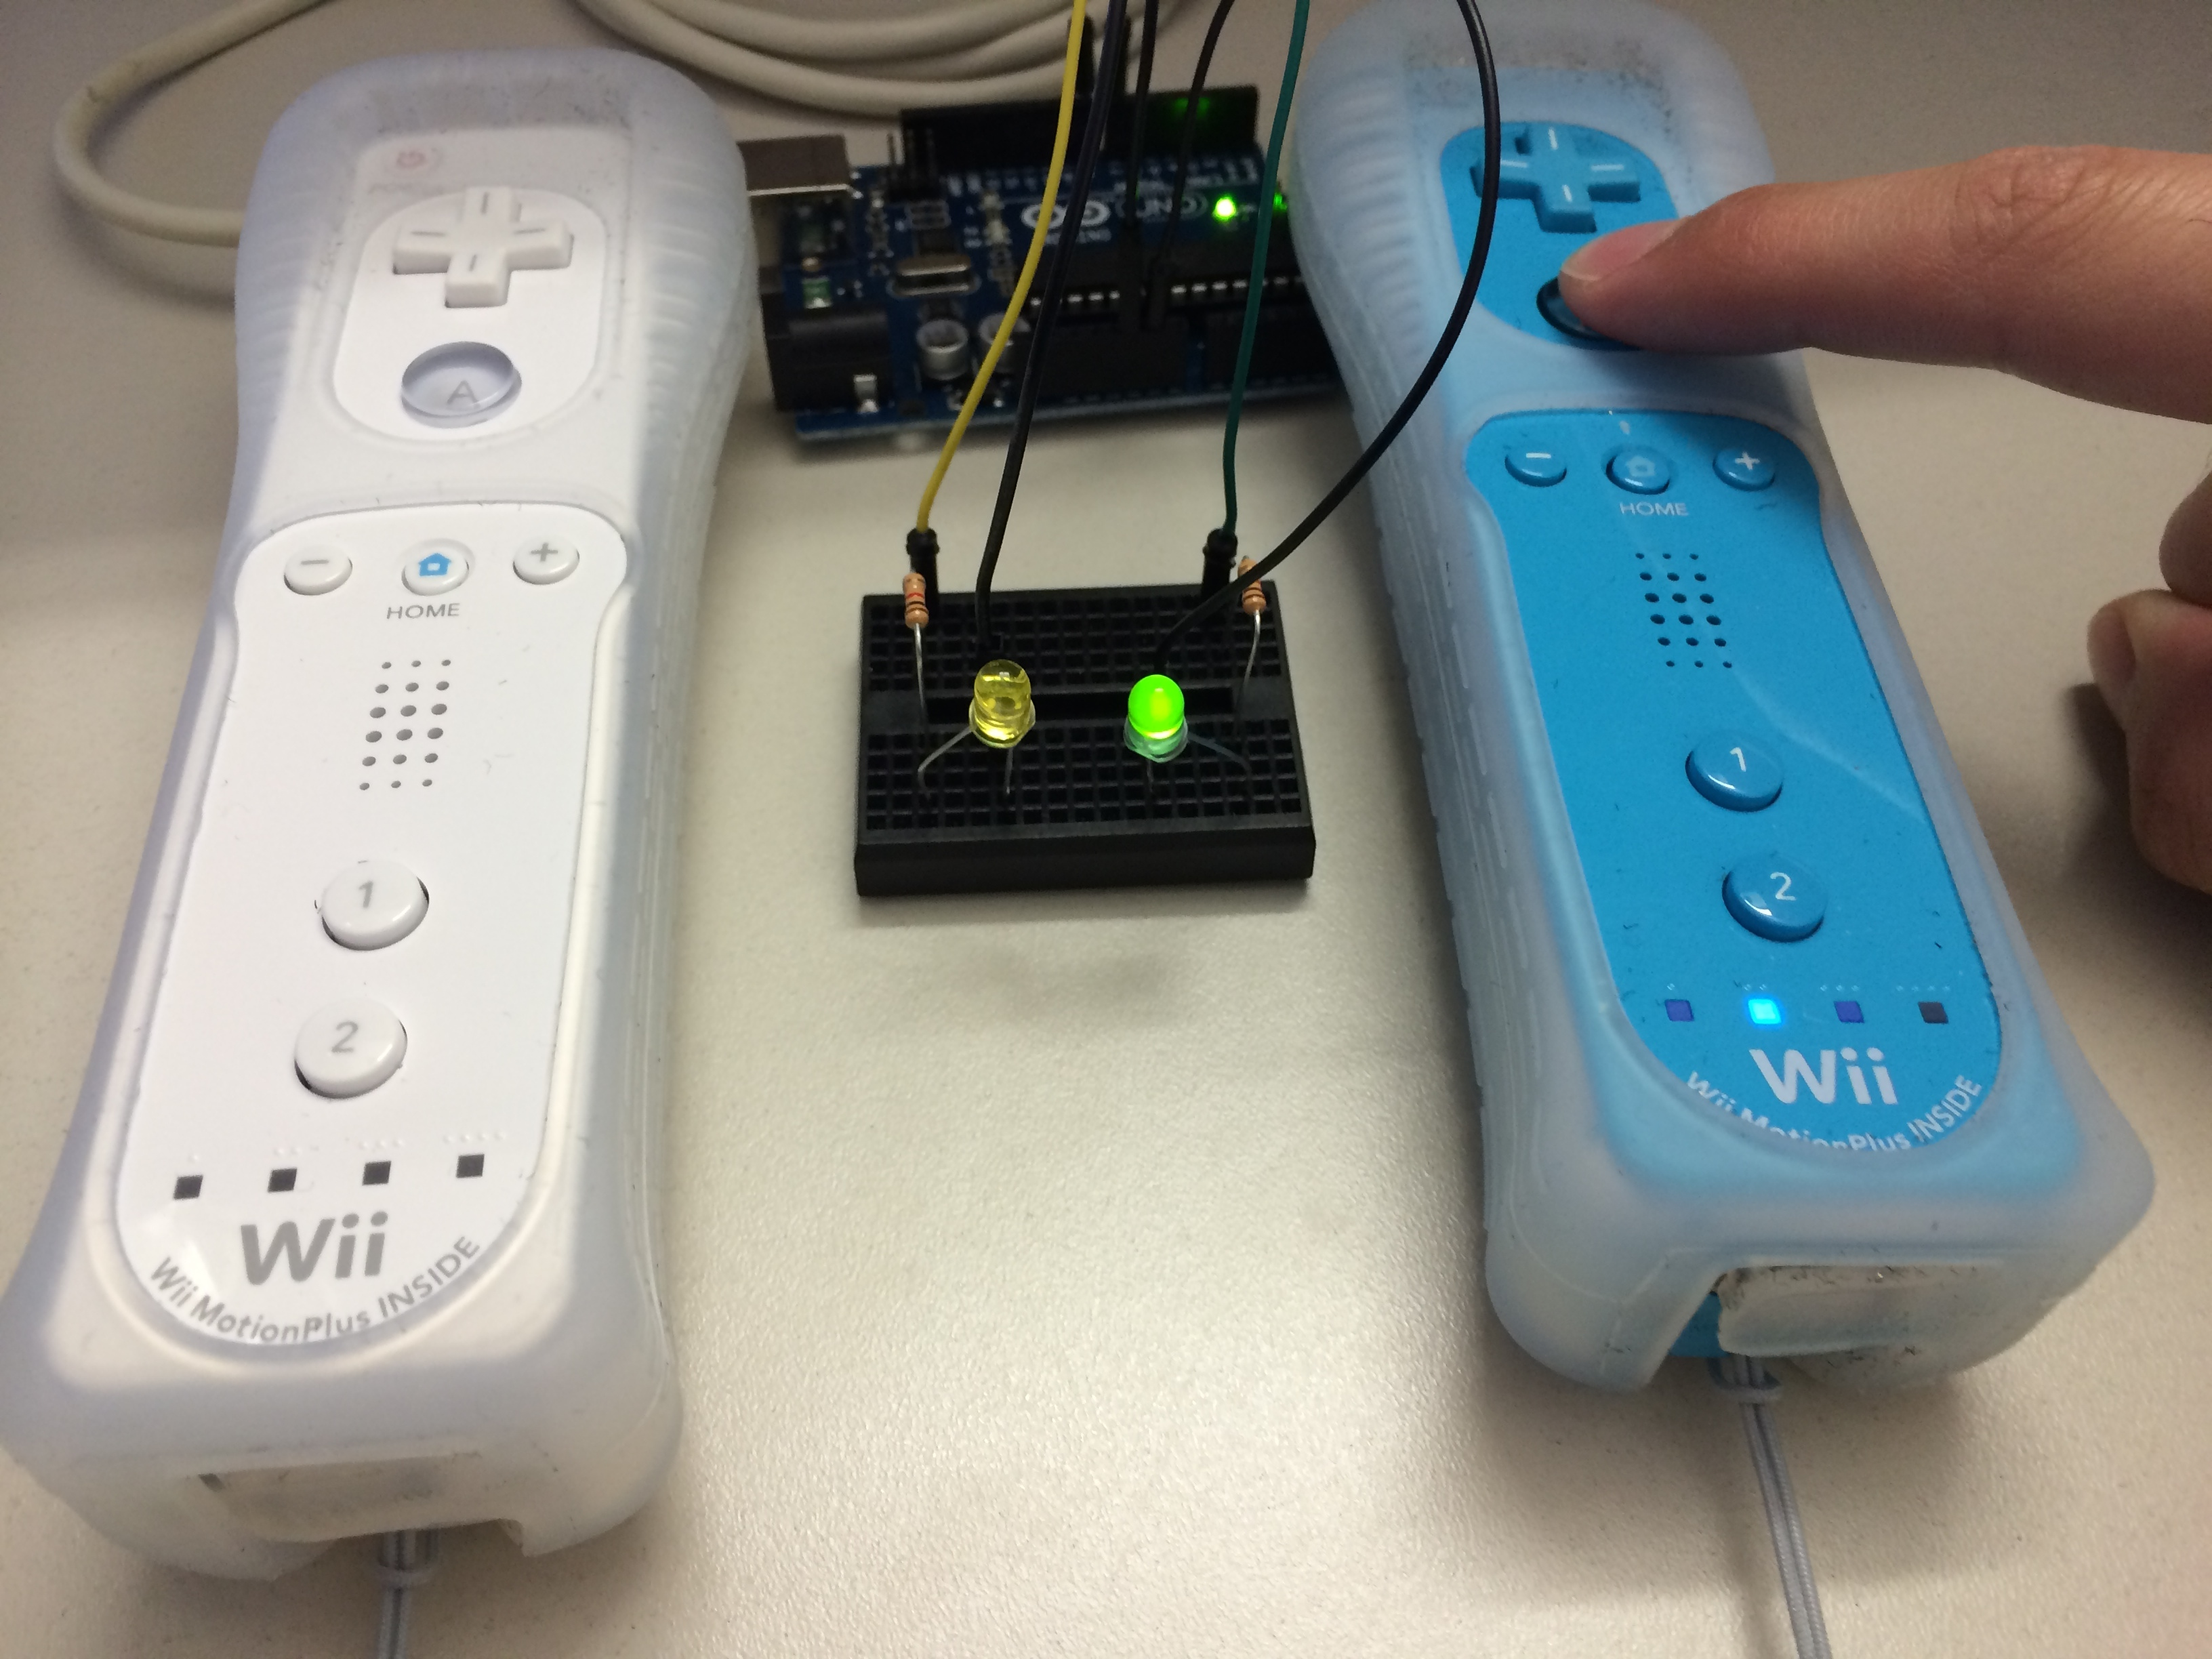
\includegraphics[height=0.4\textwidth]{wii_led.jpg}
	\caption{Turning on an LED with a Wii controller using Maxuino}

	\label{prototyping3.1}
\end{figure}

The prototype was built off of the reliable framework used in the previous experiments. Audience members would be given Wii controllers, and OSCulator and Max would process the data they generate. In order to operate lights, however, I also needed to make use of an Arduino microcontroller. This compact and versatile board could be easily programmed to control multiple actuators. After installing a library called Maxuino\footnote{\url{http://www.maxuino.org}}, I was able to easily send instructions to the Arduino from the Max environment. As an initial test, I pulled button-press data from one Wii controller and connected the Arduino to an LED; I was successfully able to illuminate the LED by pressing the controller's A button, as shown in Figure \ref{prototyping3.1}.

\begin{figure}
	\centering

	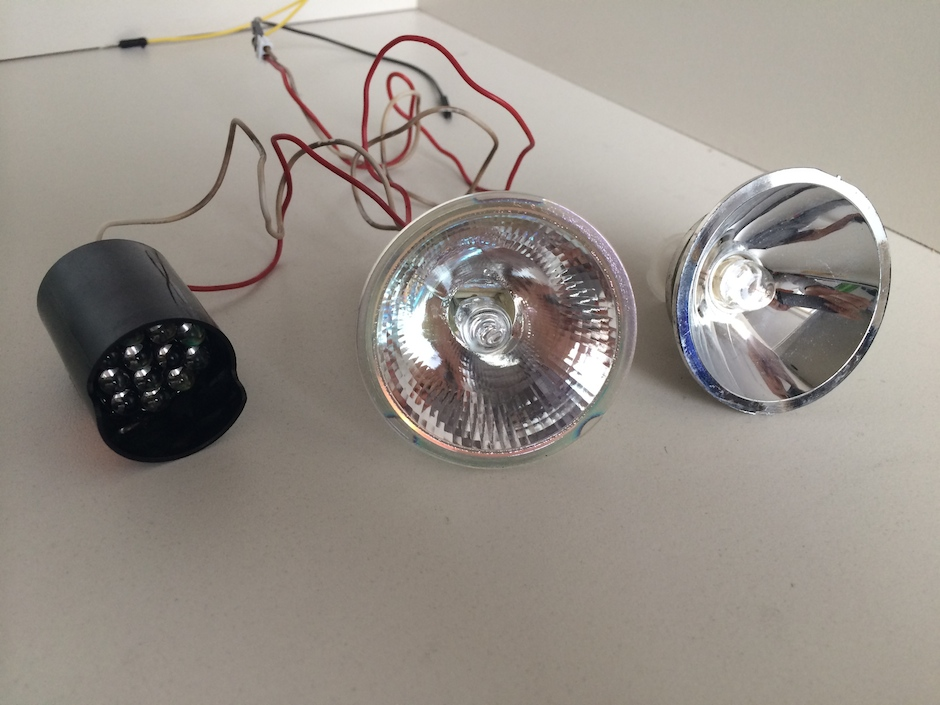
\includegraphics[height=0.4\textwidth]{light_1.jpg}
	\caption{Testing different types of lights}

	\label{prototyping3.2}
\end{figure}

Next, I tested three different light bulbs -- two incandescent bulbs with different power ratings and one amber LED bulb (see Figure \ref{prototyping3.2}). Both incandescent bulbs, once turned on, provided a great deal of brightness; however, the high current draw and slow turn-on time made them undesirable overall. The LED bulb, on the other hand, turned on and off instantly, and it became sufficiently bright while only drawing around 80 mA. This bulb was clearly most suitable for the prototype.

\begin{figure}
	\centering

	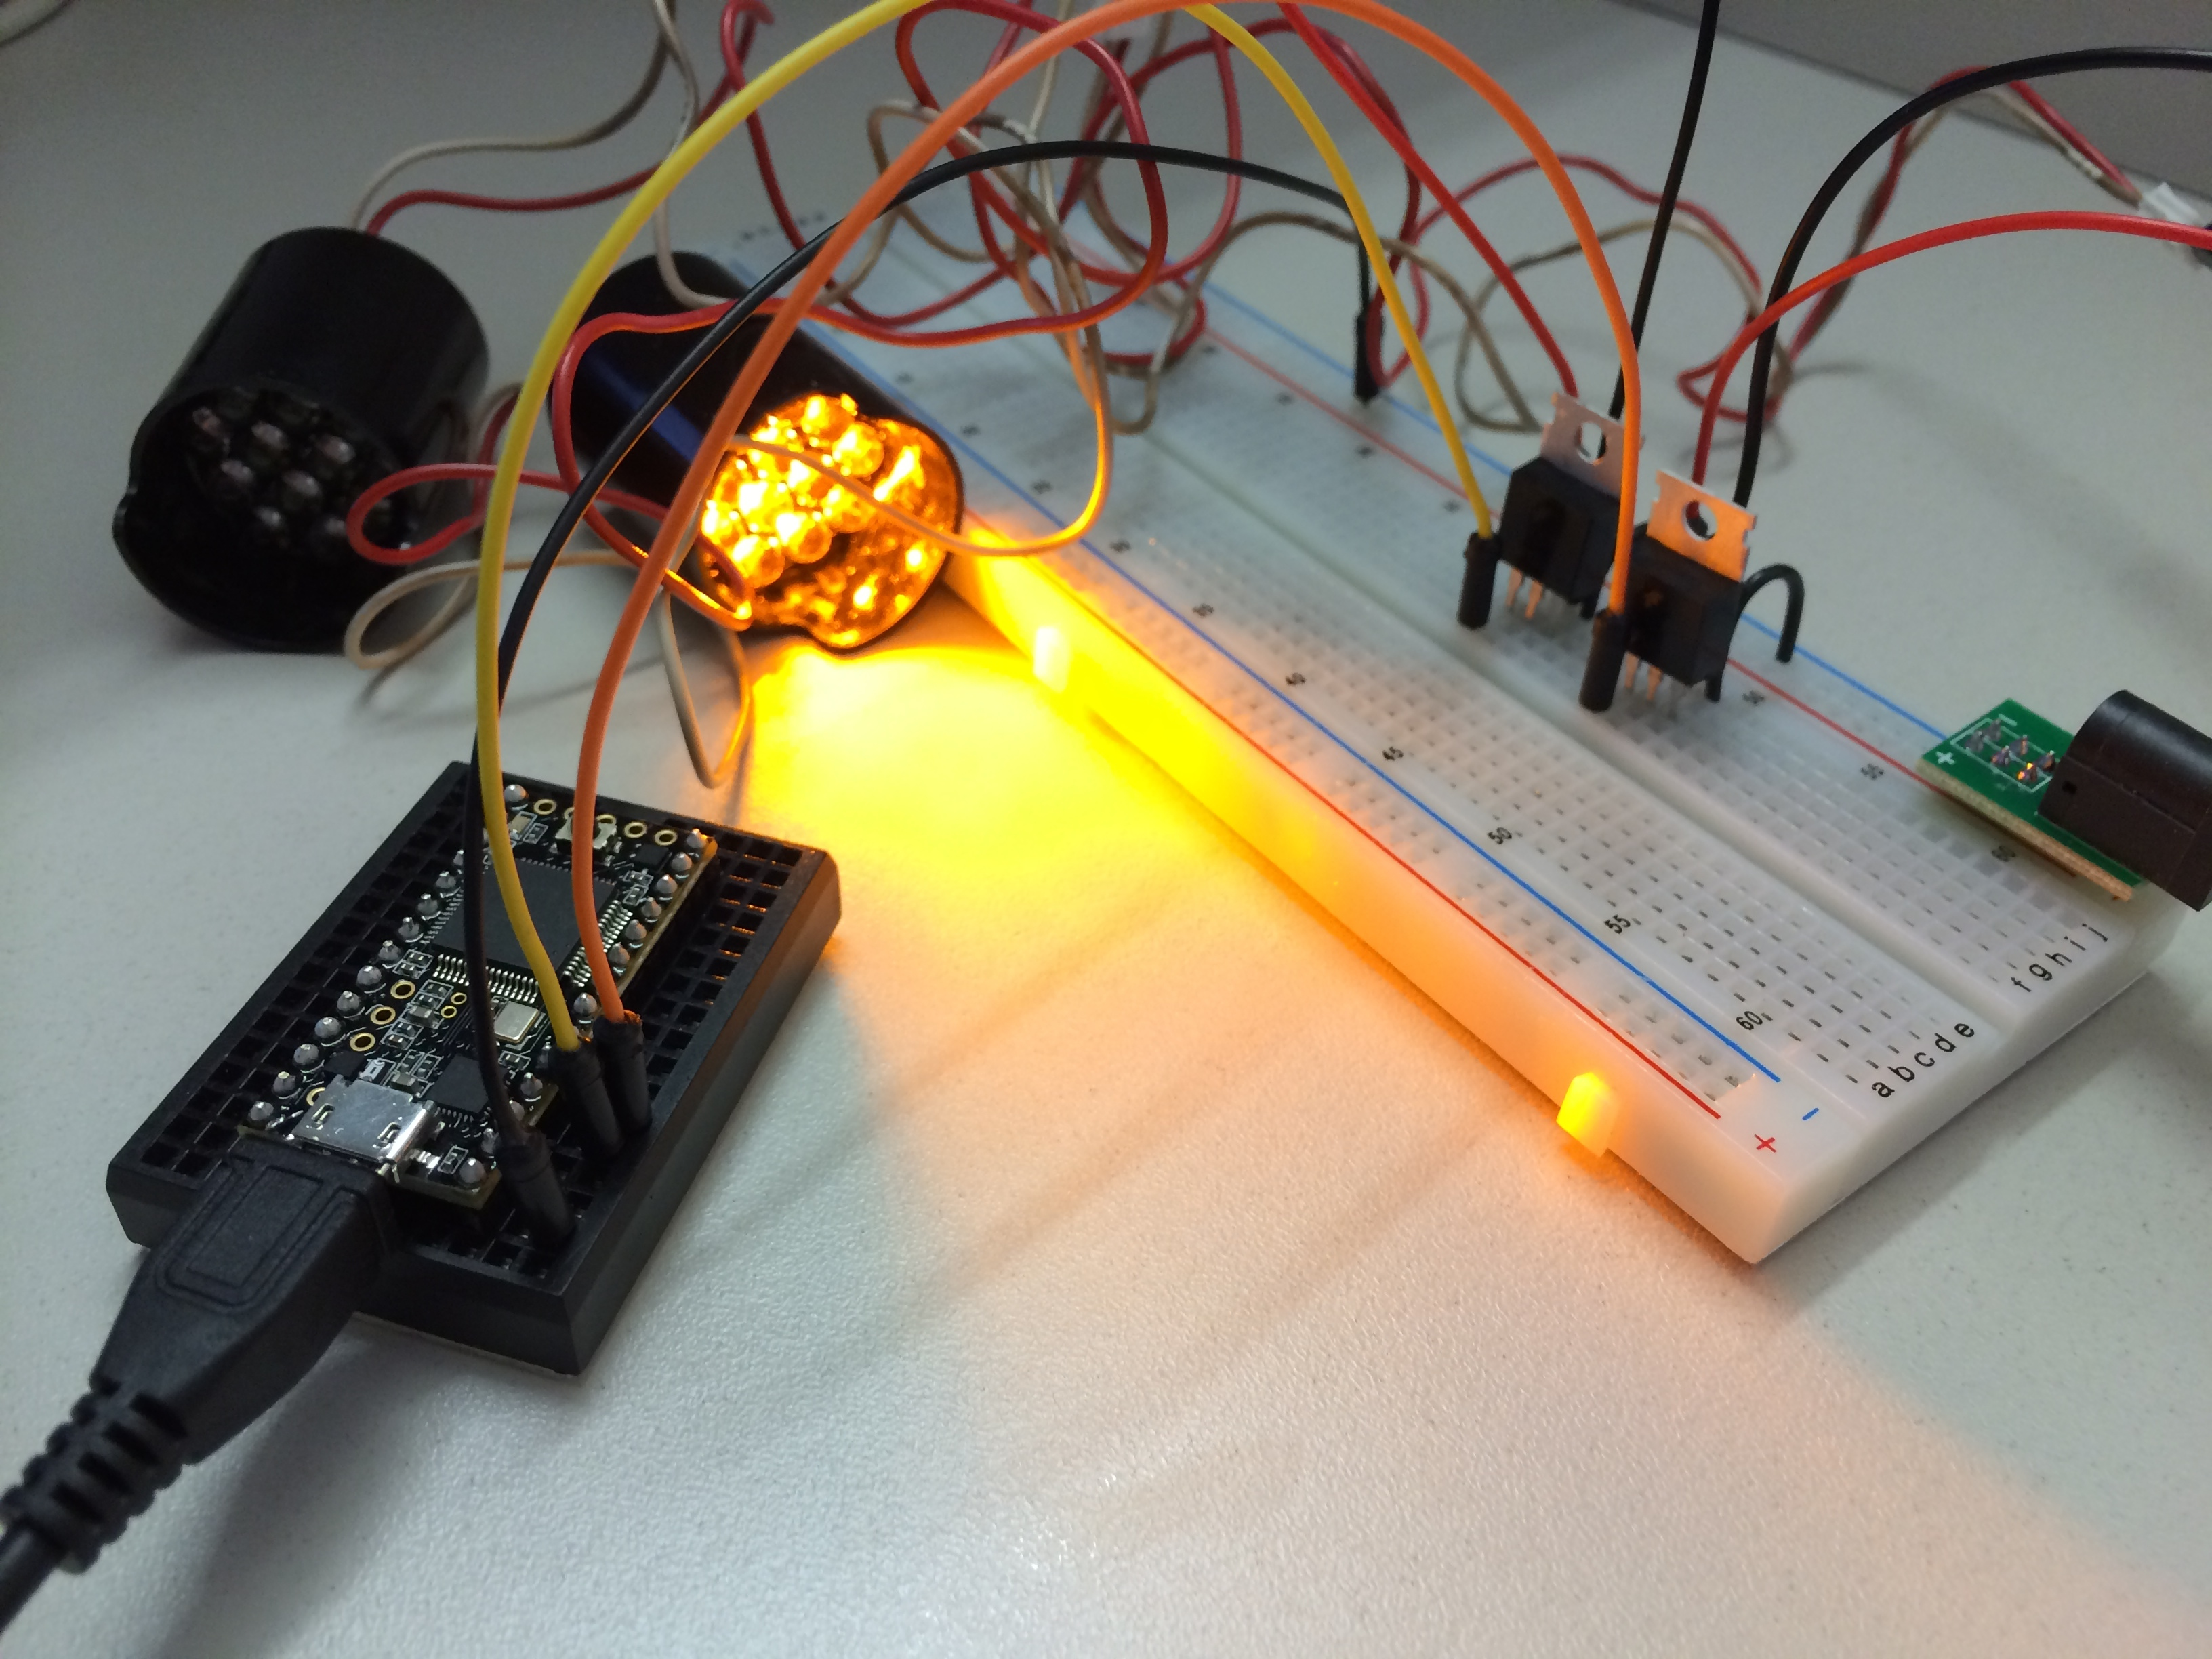
\includegraphics[height=0.4\textwidth]{light_2.jpg}
	\caption{Operating two light bulbs using transistors and Arduino}

	\label{prototyping3.3}
\end{figure}

Due to the relatively small current supplied by the microcontroller, the LED bulbs had to be controlled using a relay circuit -- that is, one where the higher-power bulbs could be controlled by lower-power signals. A power adapter was used to supply current to the bulbs, while transistors were used to control its flow. Figure \ref{prototyping3.3} shows this setup with two lights. Two Arduino pins control two transistors, thereby allowing each bulb to be turned on and off independently. By incorporating Maxuino, I was able to activate each bulb using a Wii controller.

While previous prototypes were limited to seven users, I felt that, to have a proper impact in a real concert setting, this experiment needed more participants. Since one computer can only connect to seven Wii controllers, the most straightforward solution was to use two computers. With OSCulator open on the second computer, I was able to send the controller data it received to the first computer by creating a local network. With this, I could also control the LEDs on all controllers from one computer. Thus, the maximum number of users grew to fourteen.

\begin{figure}
	\centering

	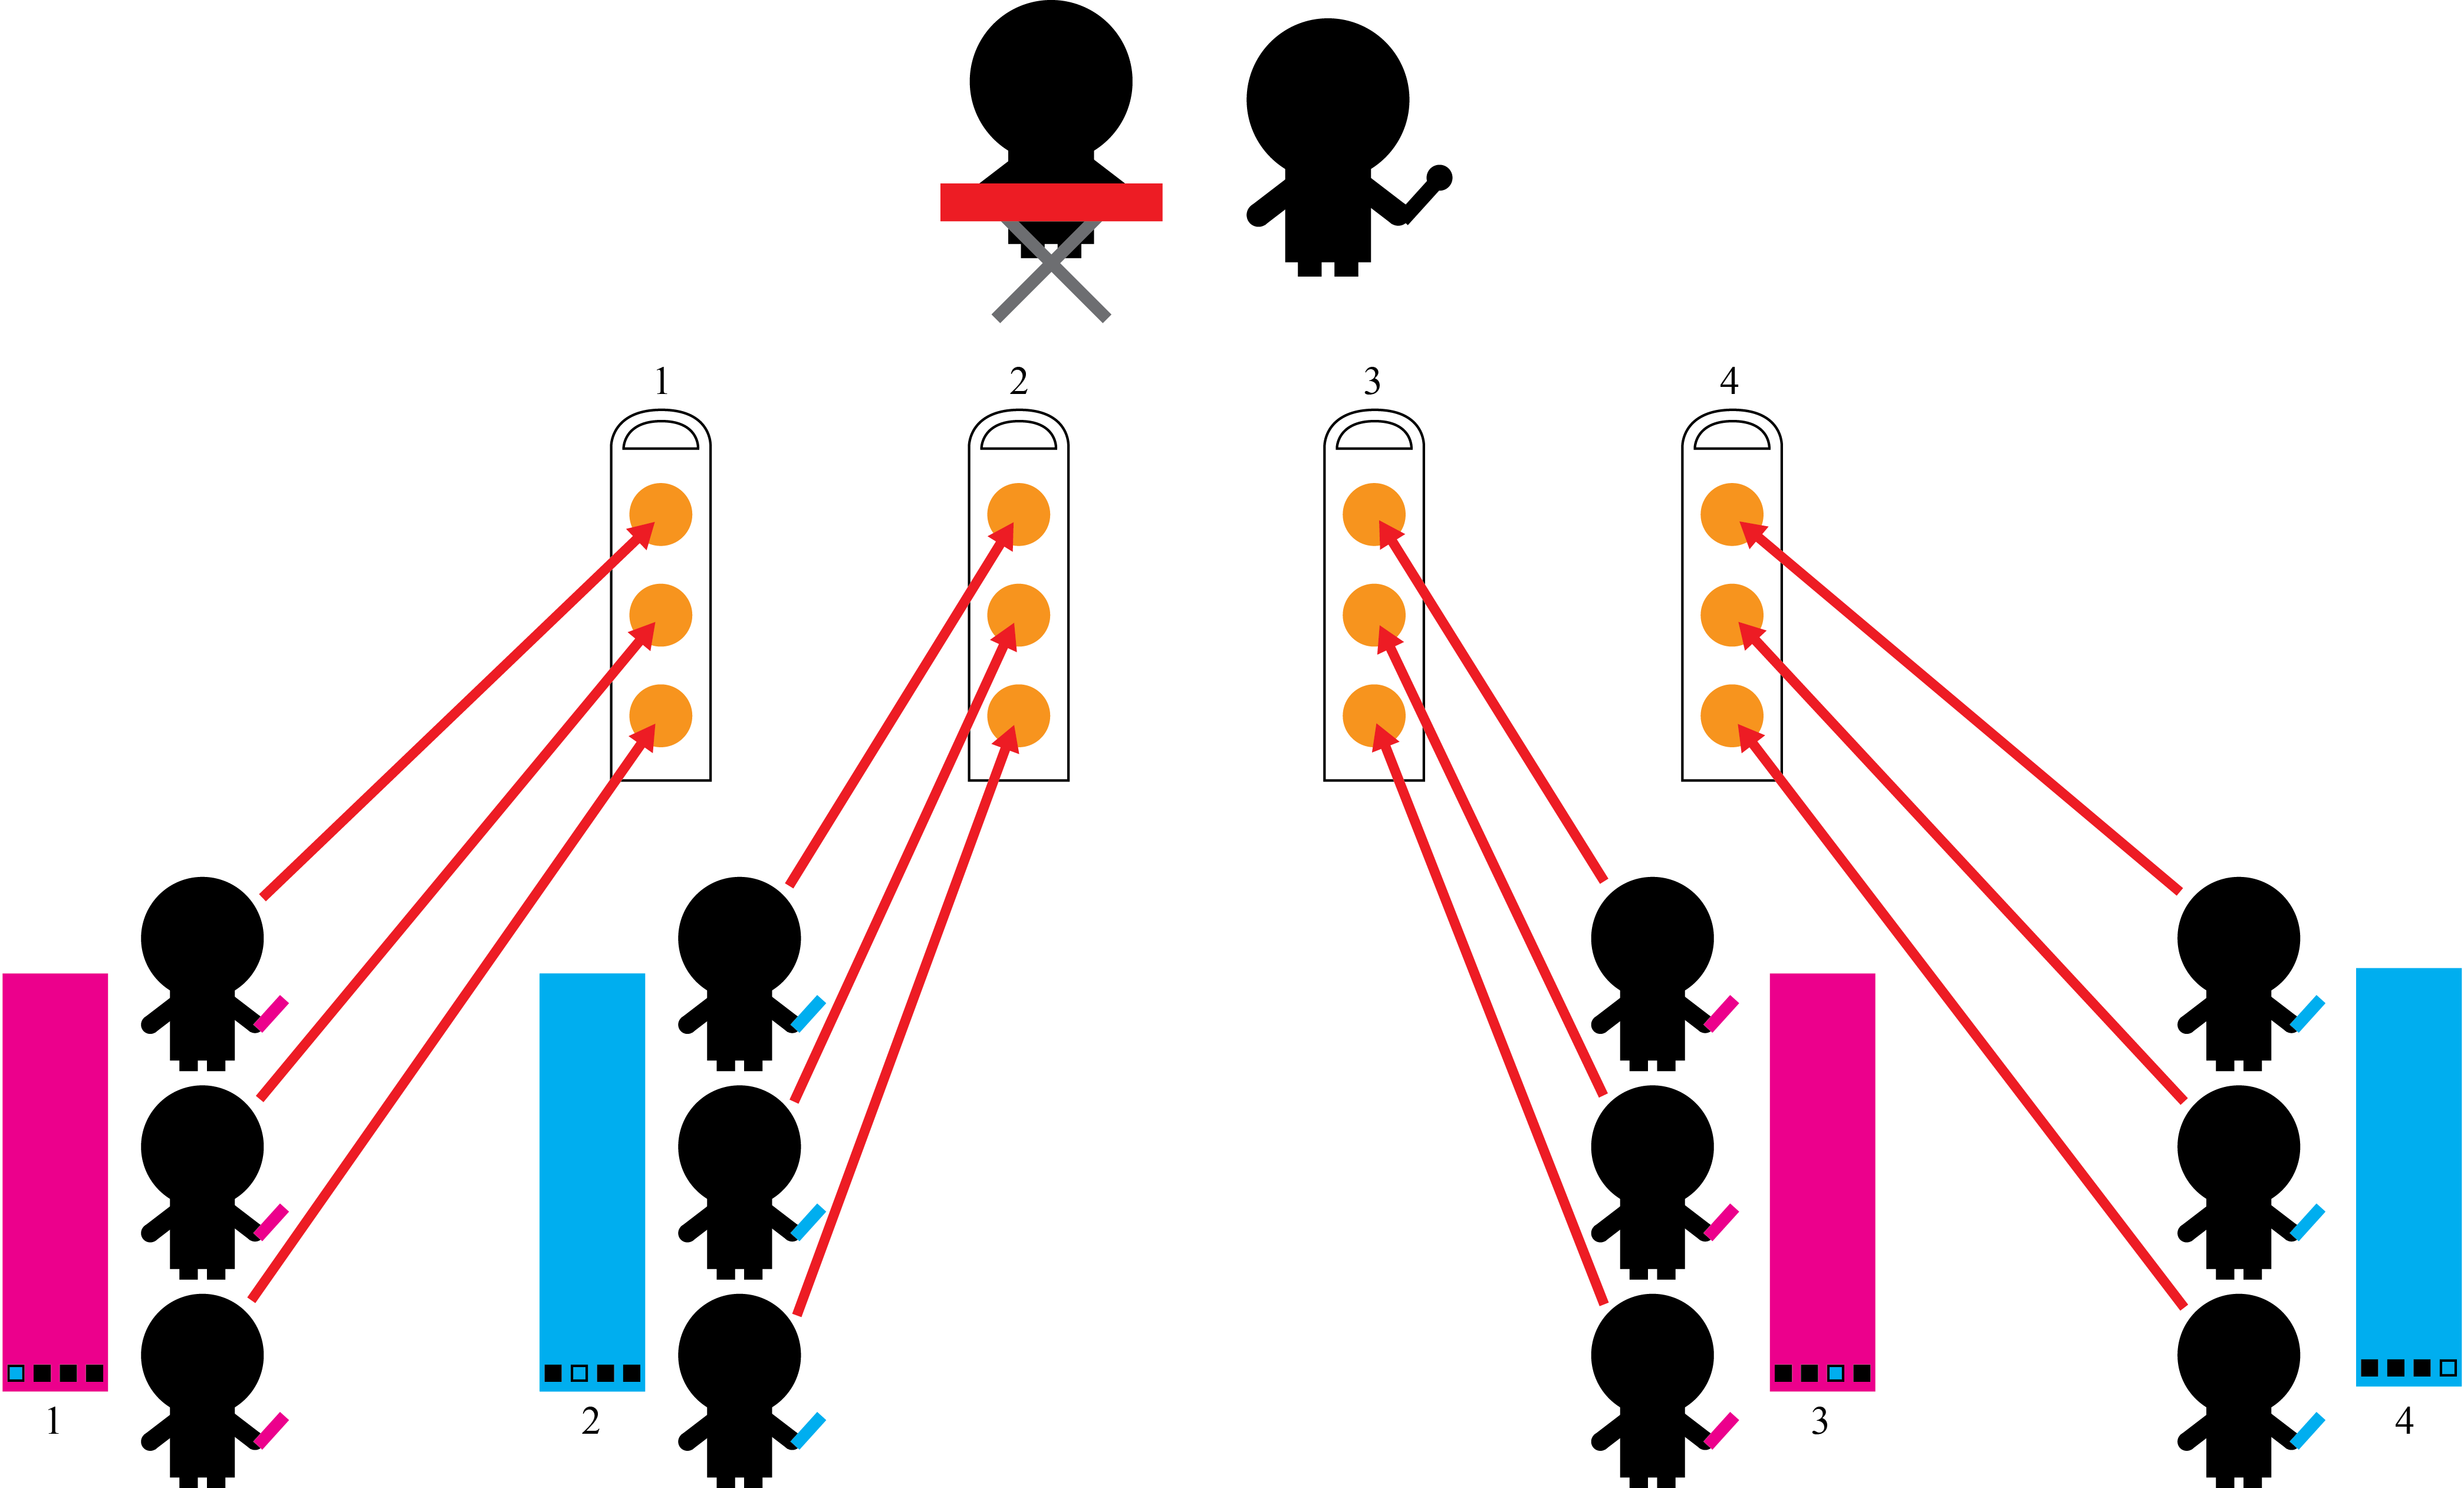
\includegraphics[width=\textwidth]{p3_diagram.png}
	\caption{Wii controller LEDs indicate each user's corresponding lamp}

	\label{prototyping3.13}
\end{figure}

Now that the primary hardware and its limitations had been established, the system could be designed with greater detail. I wanted the lights to be spread across the stage, but it was important that users could quickly identify which bulb was in their control. The Wii controller provided a solution -- namely, its four LEDs. If the lights were divided into four sections installed uniformly across the stage, a controller could indicate which section contained its paired light by illuminating the corresponding LED. A controller with the third LED illuminated, for instance, tells the user that they control a light in the third section of the stage. Thus, to evenly distribute the lights, it was decided to place three bulbs in each section, fixing the number of users at twelve. Figure \ref{prototyping3.13} further illustrates this setup.

\begin{figure}
	\centering

	\subfloat[LED control board]{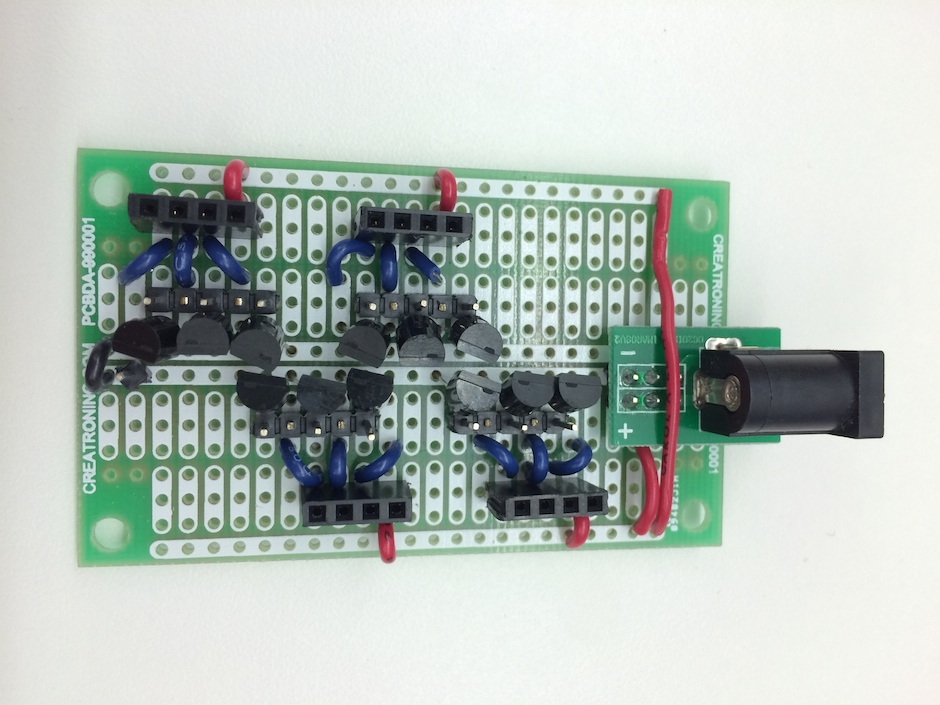
\includegraphics[height=0.36\textwidth]{board.jpg}}
	\hspace{0.1cm}
	\subfloat[Project box]{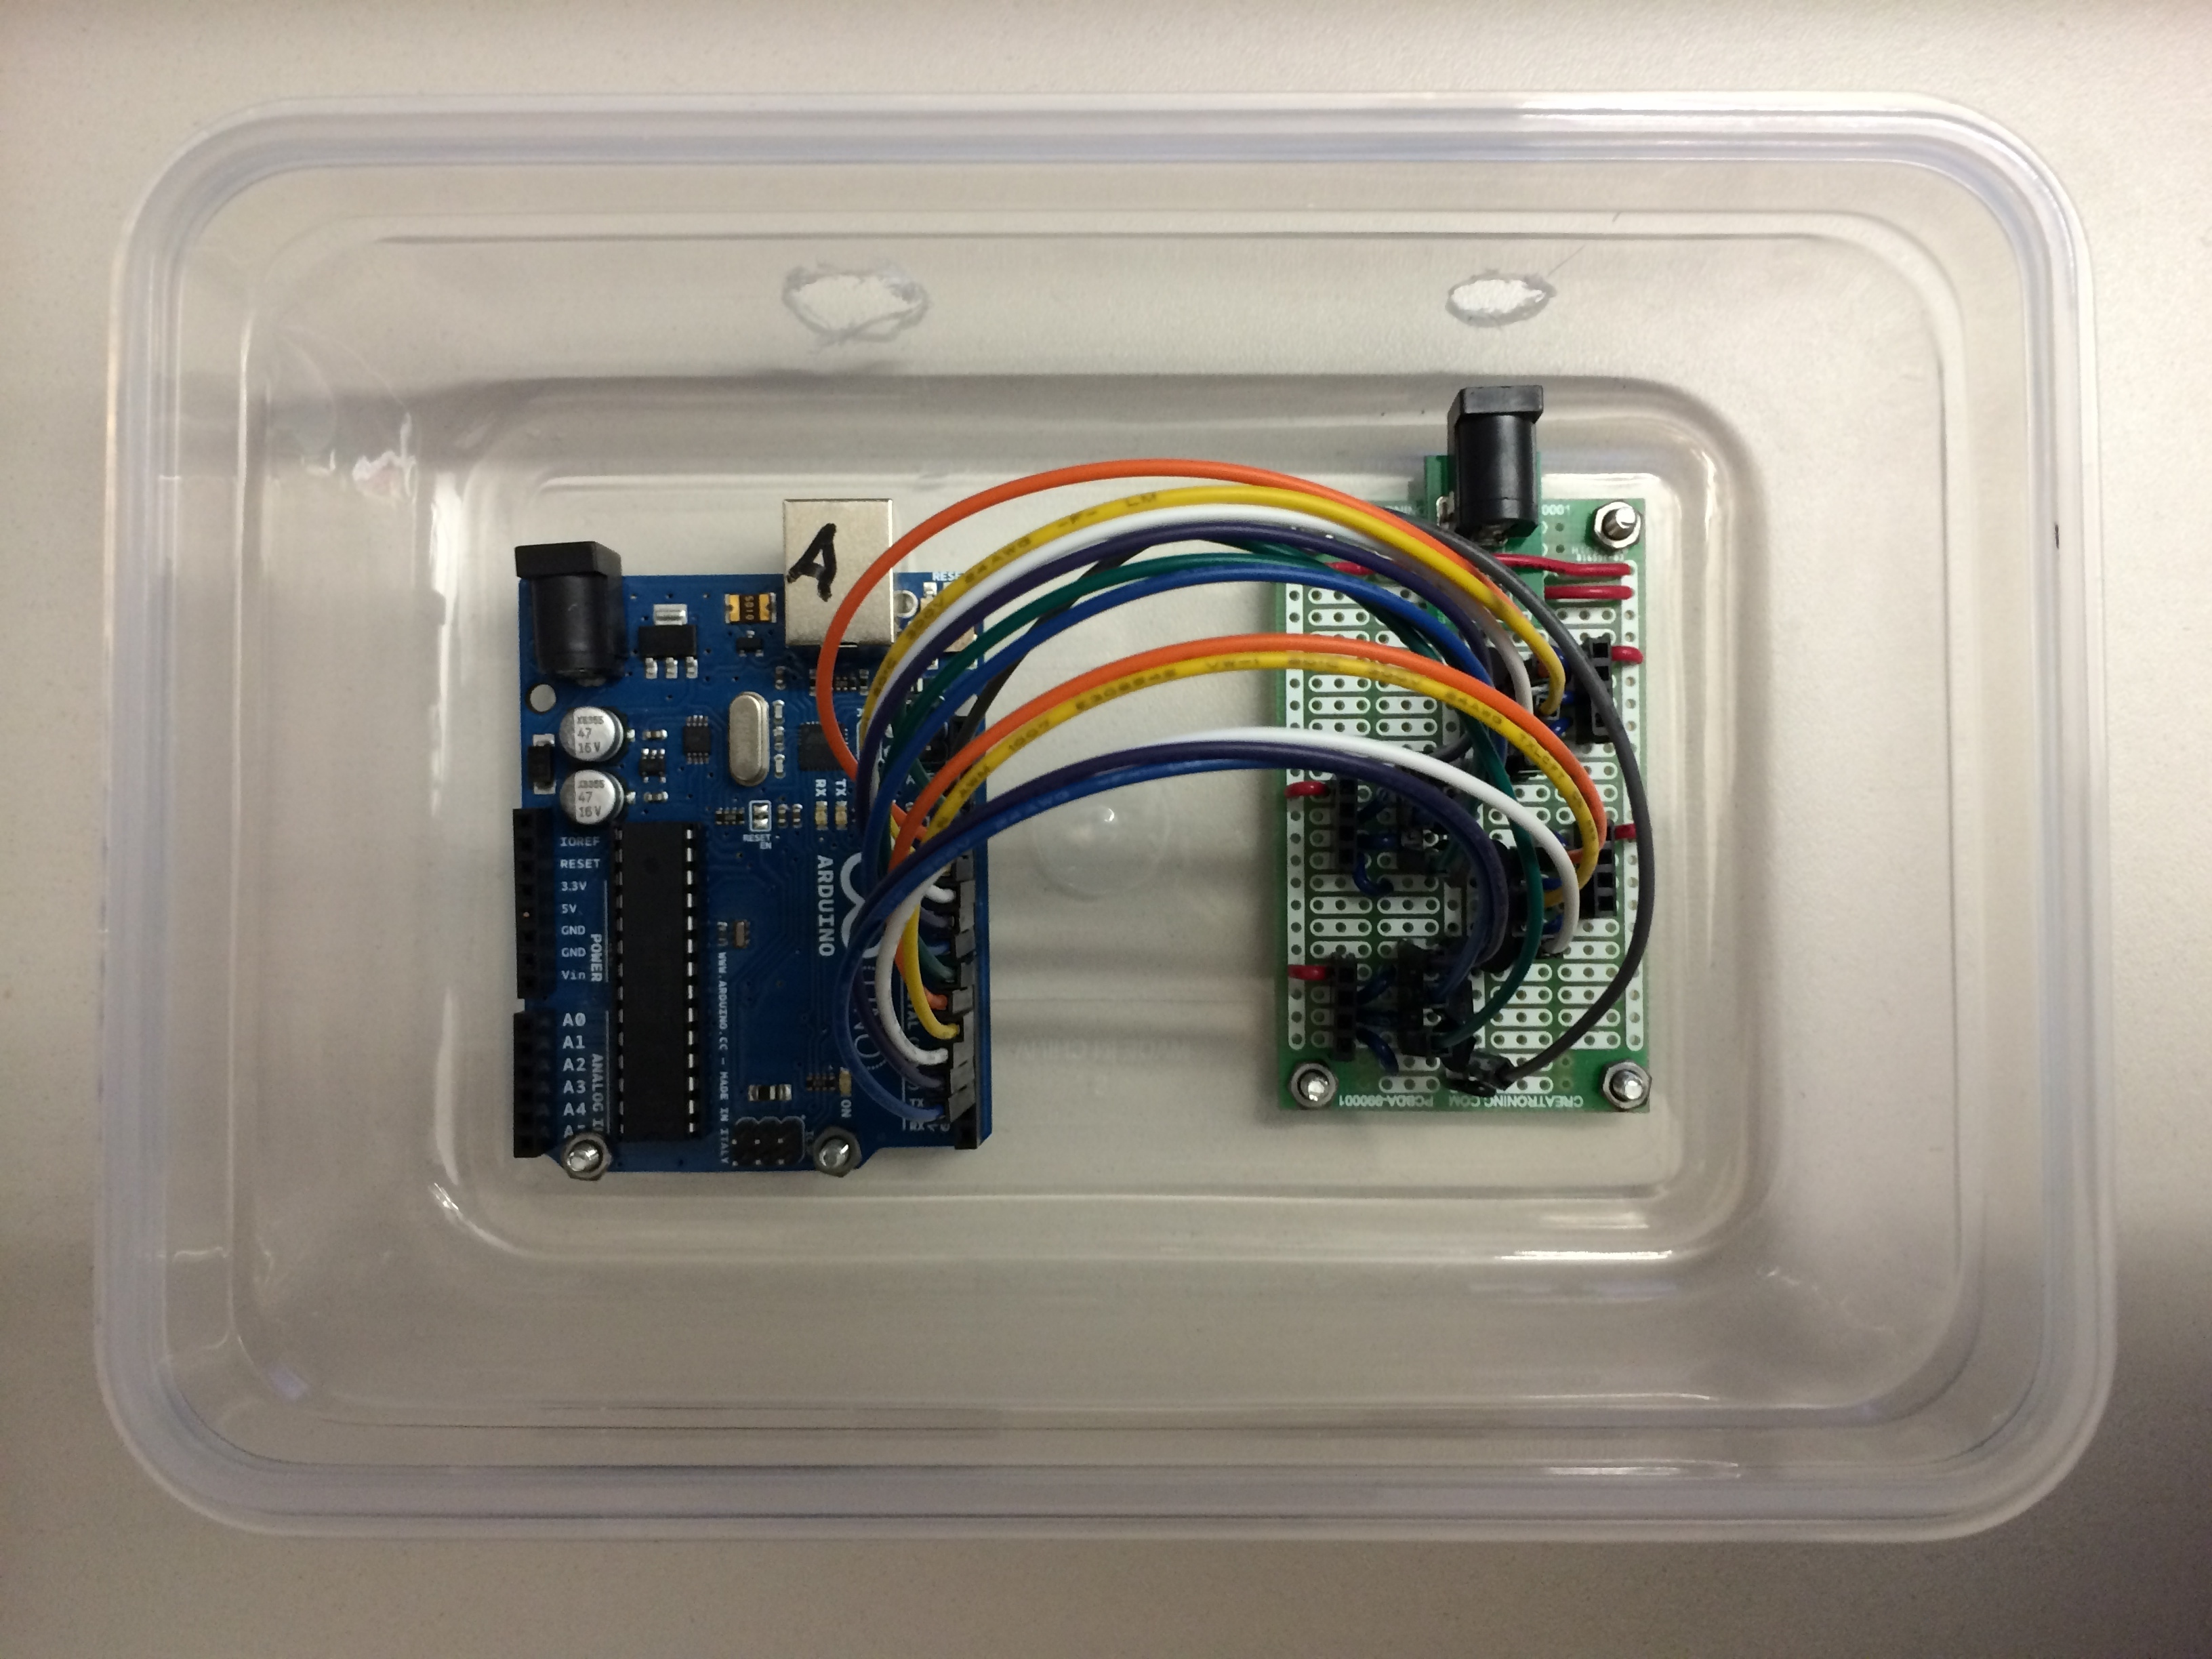
\includegraphics[height=0.36\textwidth]{electronics.jpg}}

	\caption{Electronics}

	\label{prototyping3.4}
\end{figure}

A compact circuit board was next assembled to handle the control of each bulb. The board had to contain a barrel jack for the power supply and connectors for twelve light bulbs. Smaller transistors were selected to minimize board size. Figure \ref{prototyping3.4}(a) shows the outcome. Finally, the board was installed in a plastic project box alongside the Arduino to ensure all connections remained secure while the system was in use; this is shown in Figure \ref{prototyping3.4}(b).

\begin{figure}
	\centering

	\subfloat[Laser-cut design]{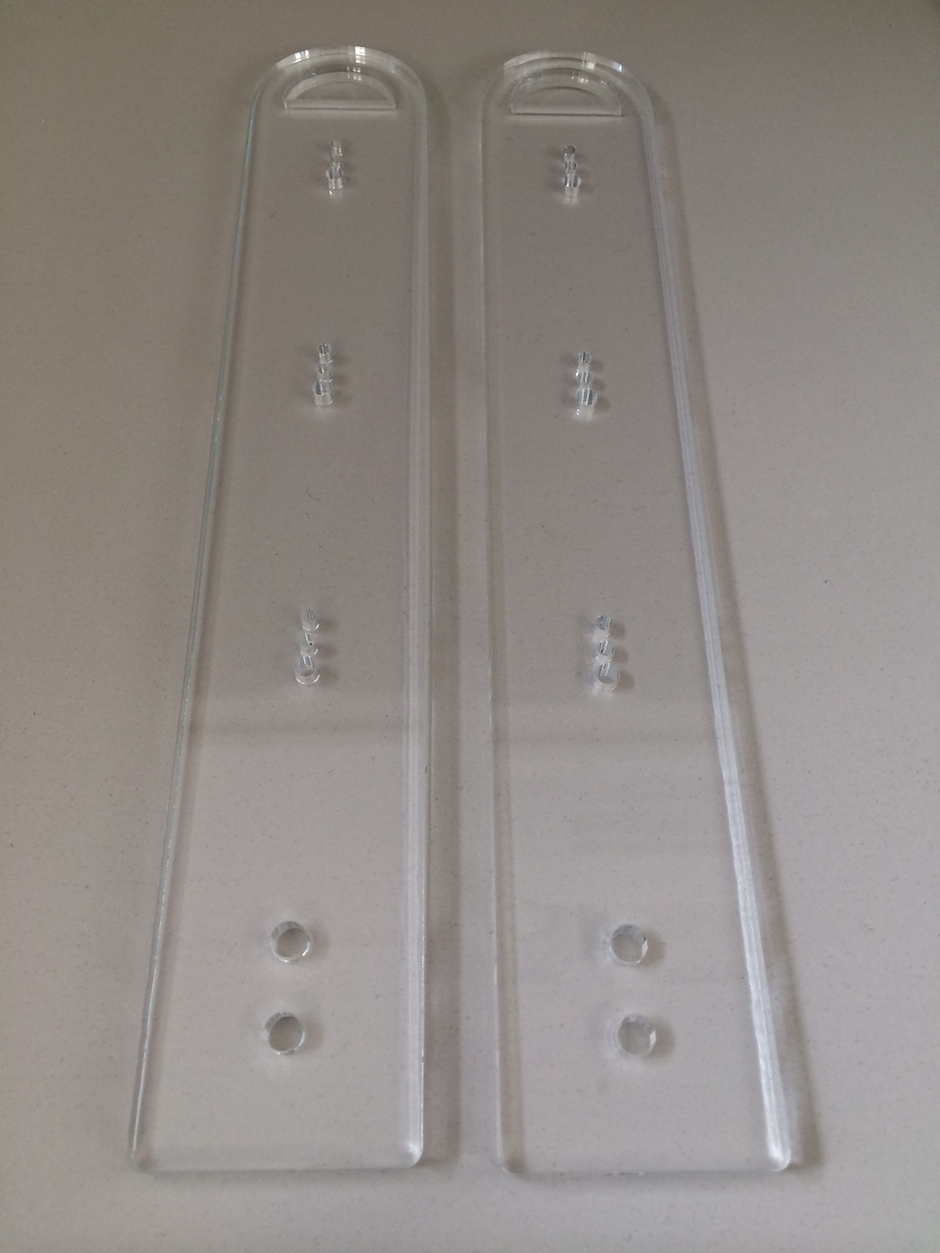
\includegraphics[height=0.45\textwidth]{rigs_1.jpg}}
	\hspace{0.1cm}
	\subfloat[Light bulbs and wire installed]{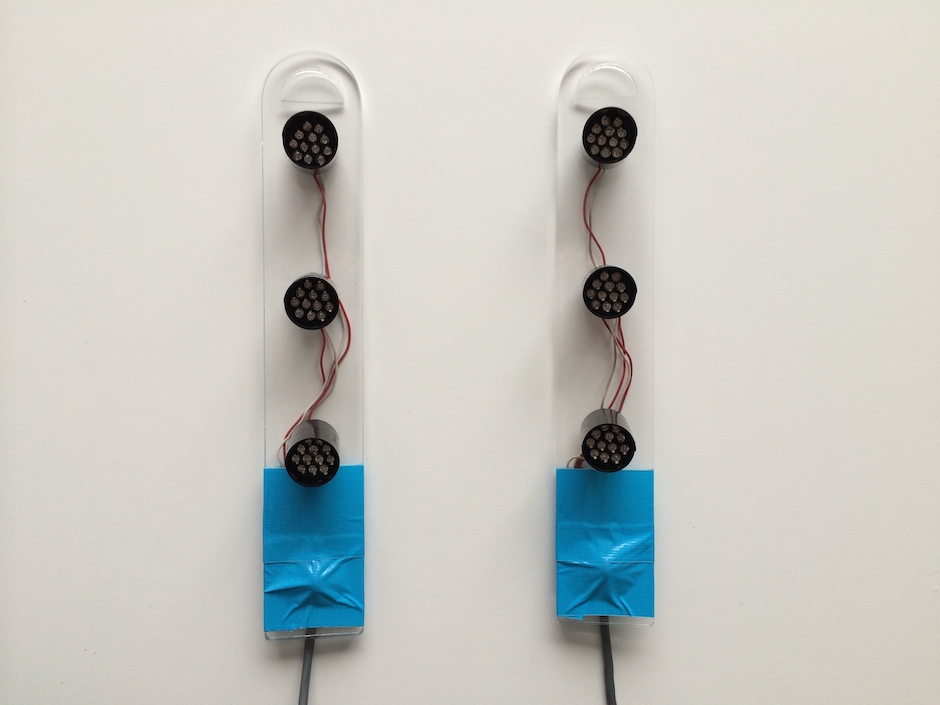
\includegraphics[height=0.45\textwidth]{rigs_2.jpg}}

	\caption{Acrylic lamps}

	\label{prototyping3.5}
\end{figure}

Simple lamps were designed to house the bulbs; four would hold three bulbs each. I decided to use acrylic, a relatively durable and accessible material that could be quickly laser cut with my design. A first version of the lamp was cut in quarter-inch-thick acrylic to ensure measurements were correct. After making some adjustments, the lamps pictured in Figure \ref{prototyping3.5} were created. A hole was placed at the top of each lamp so that they could be easily tied to or hung from something on stage. Lastly, each lamp was connected to approximately fifteen feet of wire, ending in a connector that plugs in to the circuit board's terminals.

\begin{figure}
	\centering

	\subfloat[Controller with foam cover]{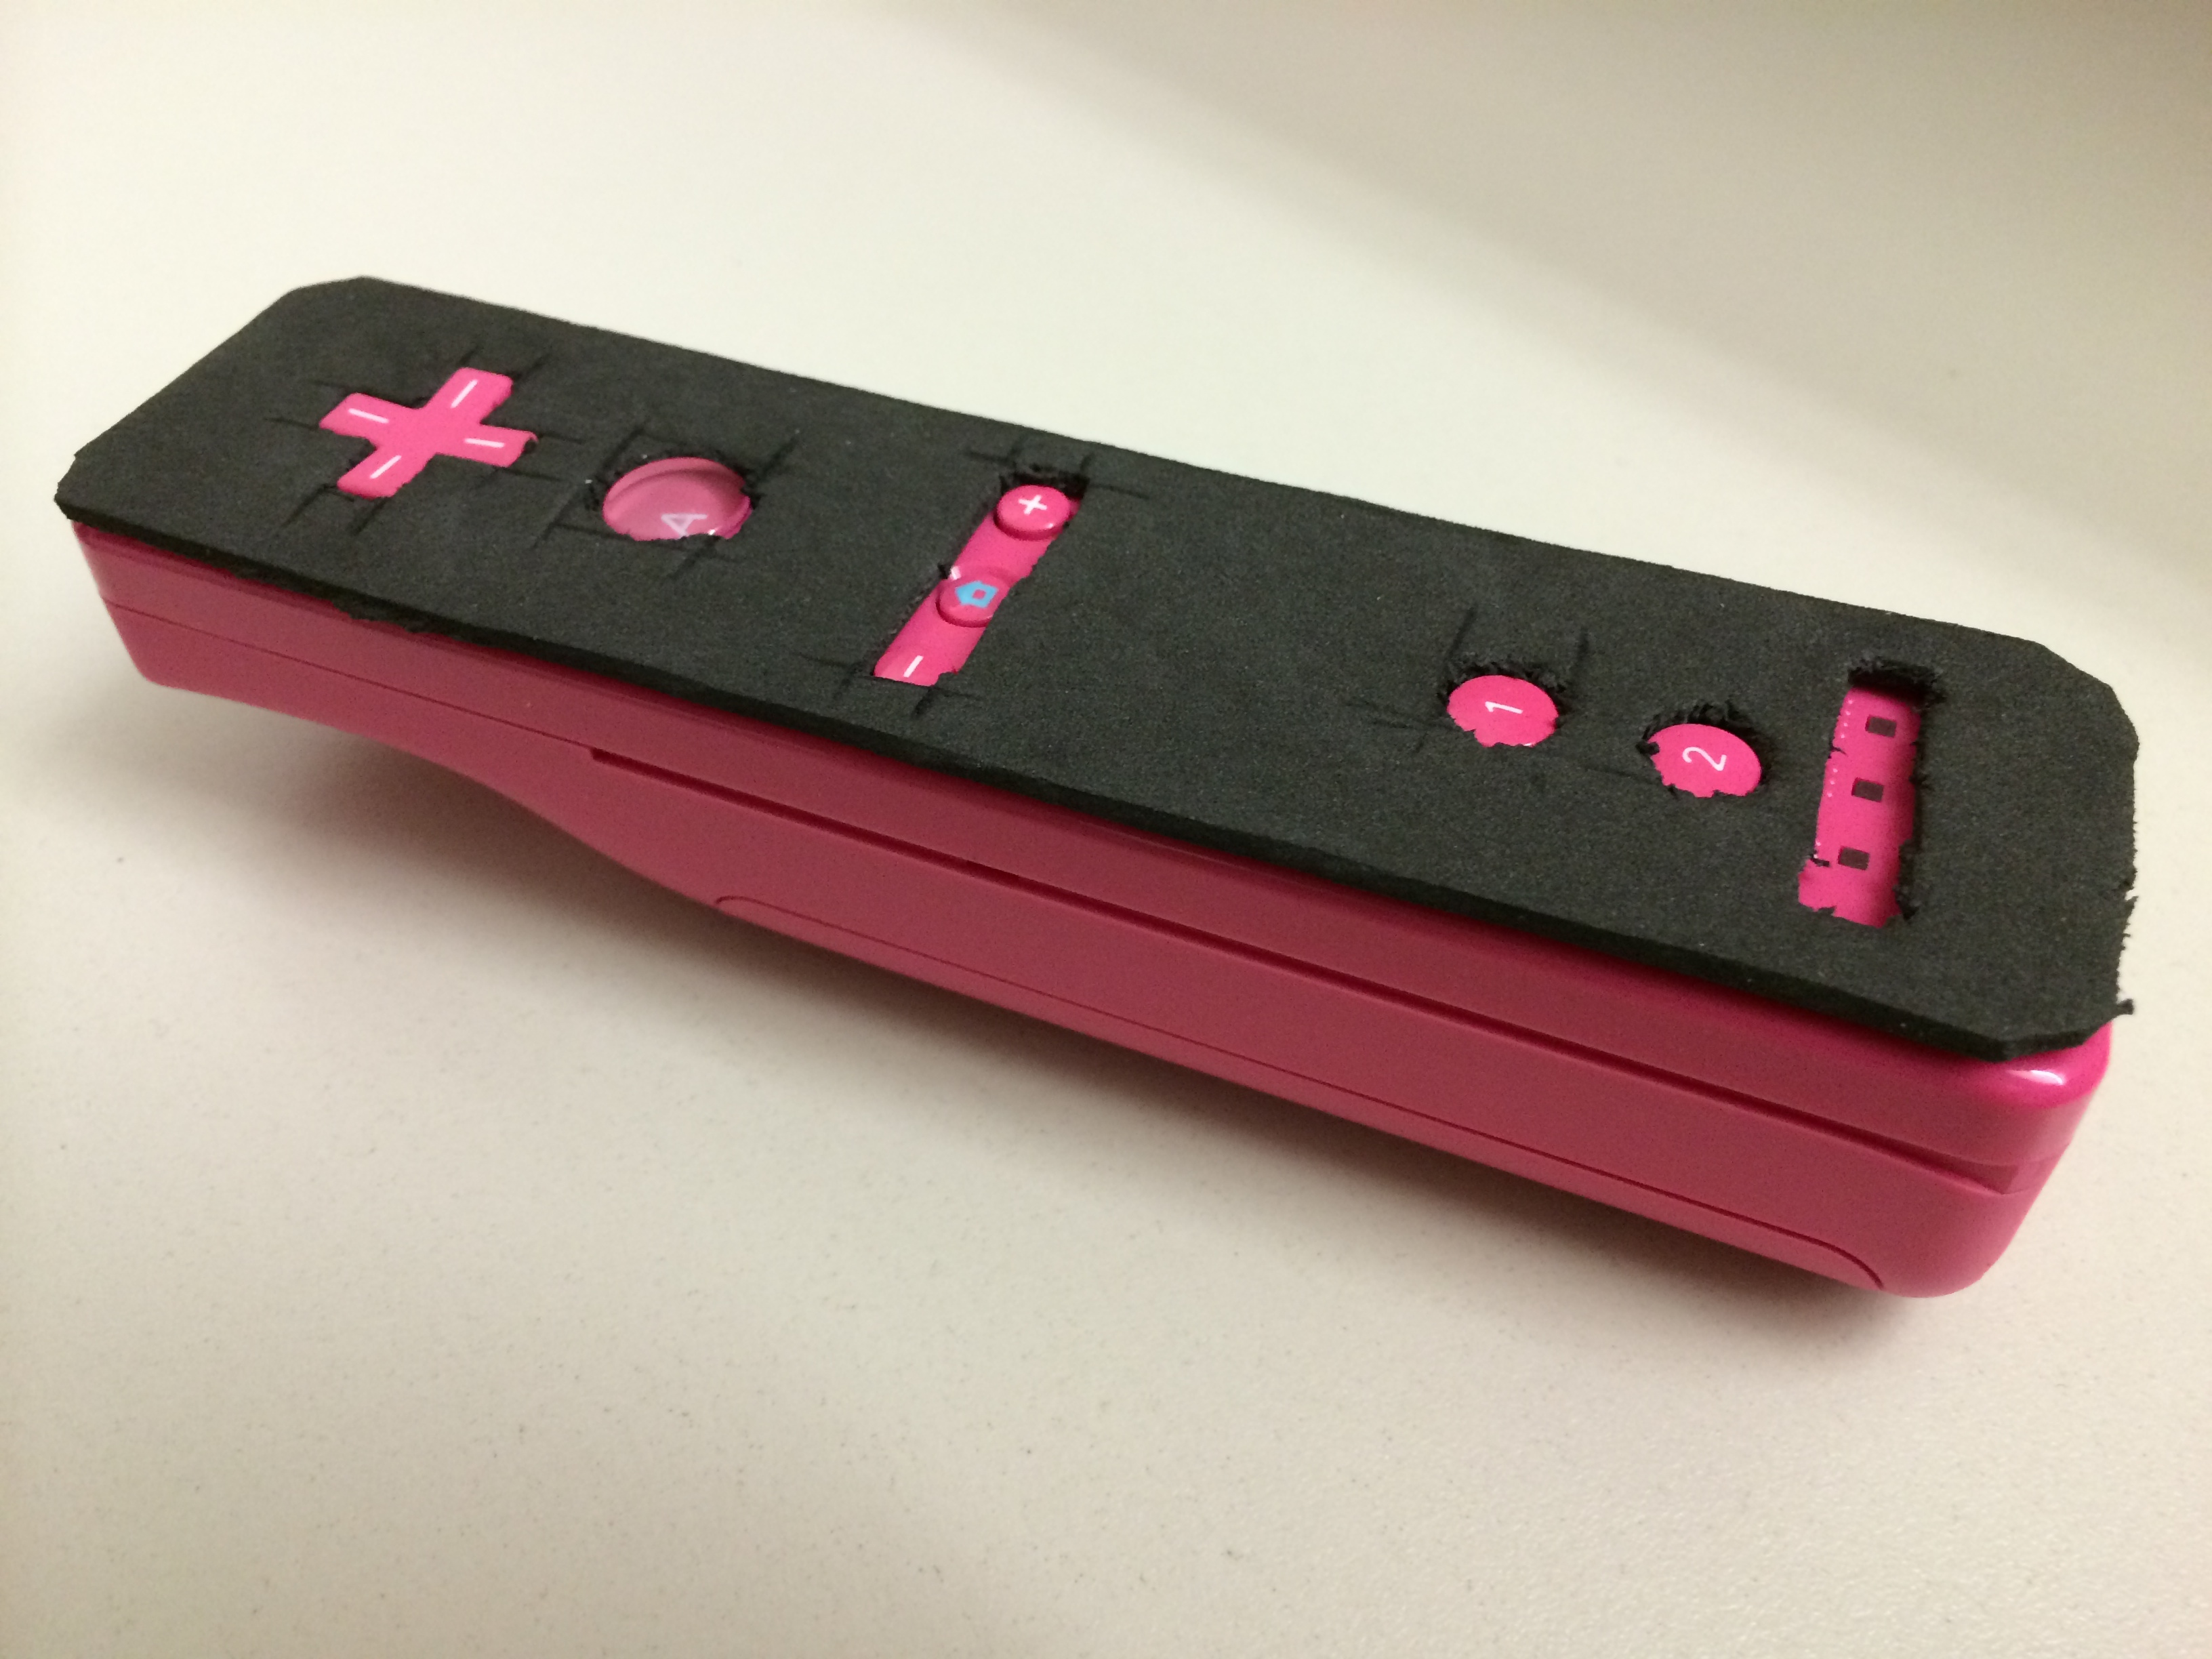
\includegraphics[height=0.36\textwidth]{wii.jpg}}
	\hspace{0.1cm}
	\subfloat[Taped controllers]{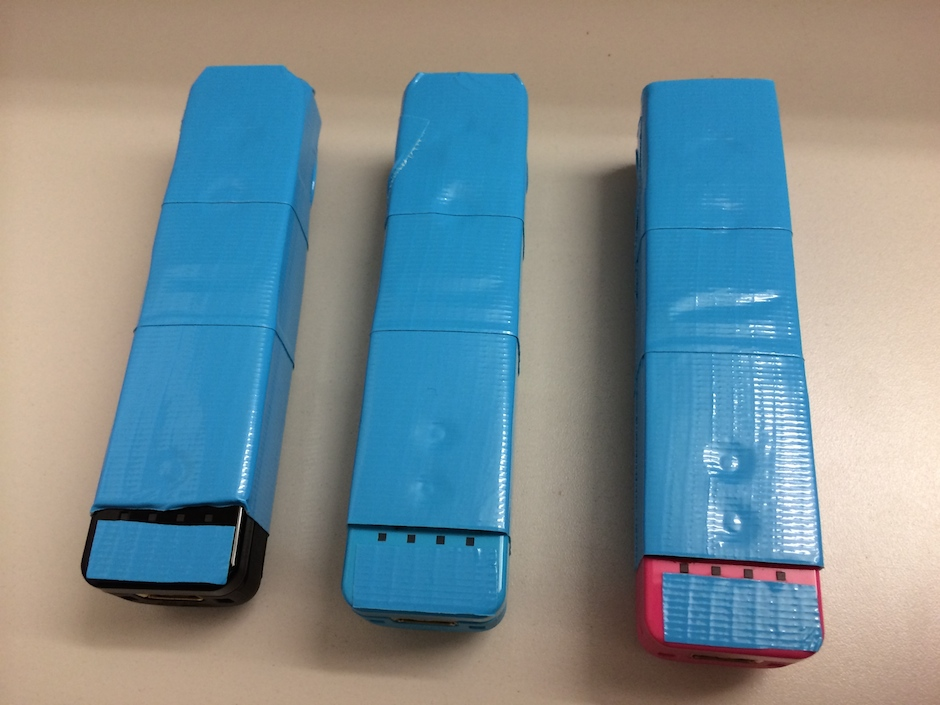
\includegraphics[height=0.36\textwidth]{wiis.jpg}}

	\caption{Preparing the Wii controllers}

	\label{prototyping3.6}
\end{figure}

Next, a Max patcher was created to pull data from all twelve Wii controllers and control all twelve lights. But how exactly would a user turn on their light? It was decided that the bulbs would be activated by performing a clapping motion with the controller. Out of the methods tested with the last prototype, I felt that this made the most sense with the system: simply clap your controller against your palm to momentarily illuminate your light. This input method was generally well received by users of the previous prototype, but it received some criticisms. For instance, users felt the visuals did not respond quickly enough to their claps; a quick test with the LED bulbs indicated that such latency would not be an issue here. Some Prototype \#2 users also noted discomfort when performing the clapping motion. To address this, a foam cover was added to the Wii controllers, and they were wrapped in tape (see Figure \ref{prototyping3.6}). This also solved another problem that emerged in the previous experiment: some users were distracted by the controller's buttons. By covering the buttons, users would not presume that they served a function. An additional method of visual feedback was added at this stage as well. While one LED would remain illuminated at all times, a registered clap input would cause all four LEDs on a user's controller to momentarily flash in sync with their connected light on stage.

\begin{figure}
	\centering

	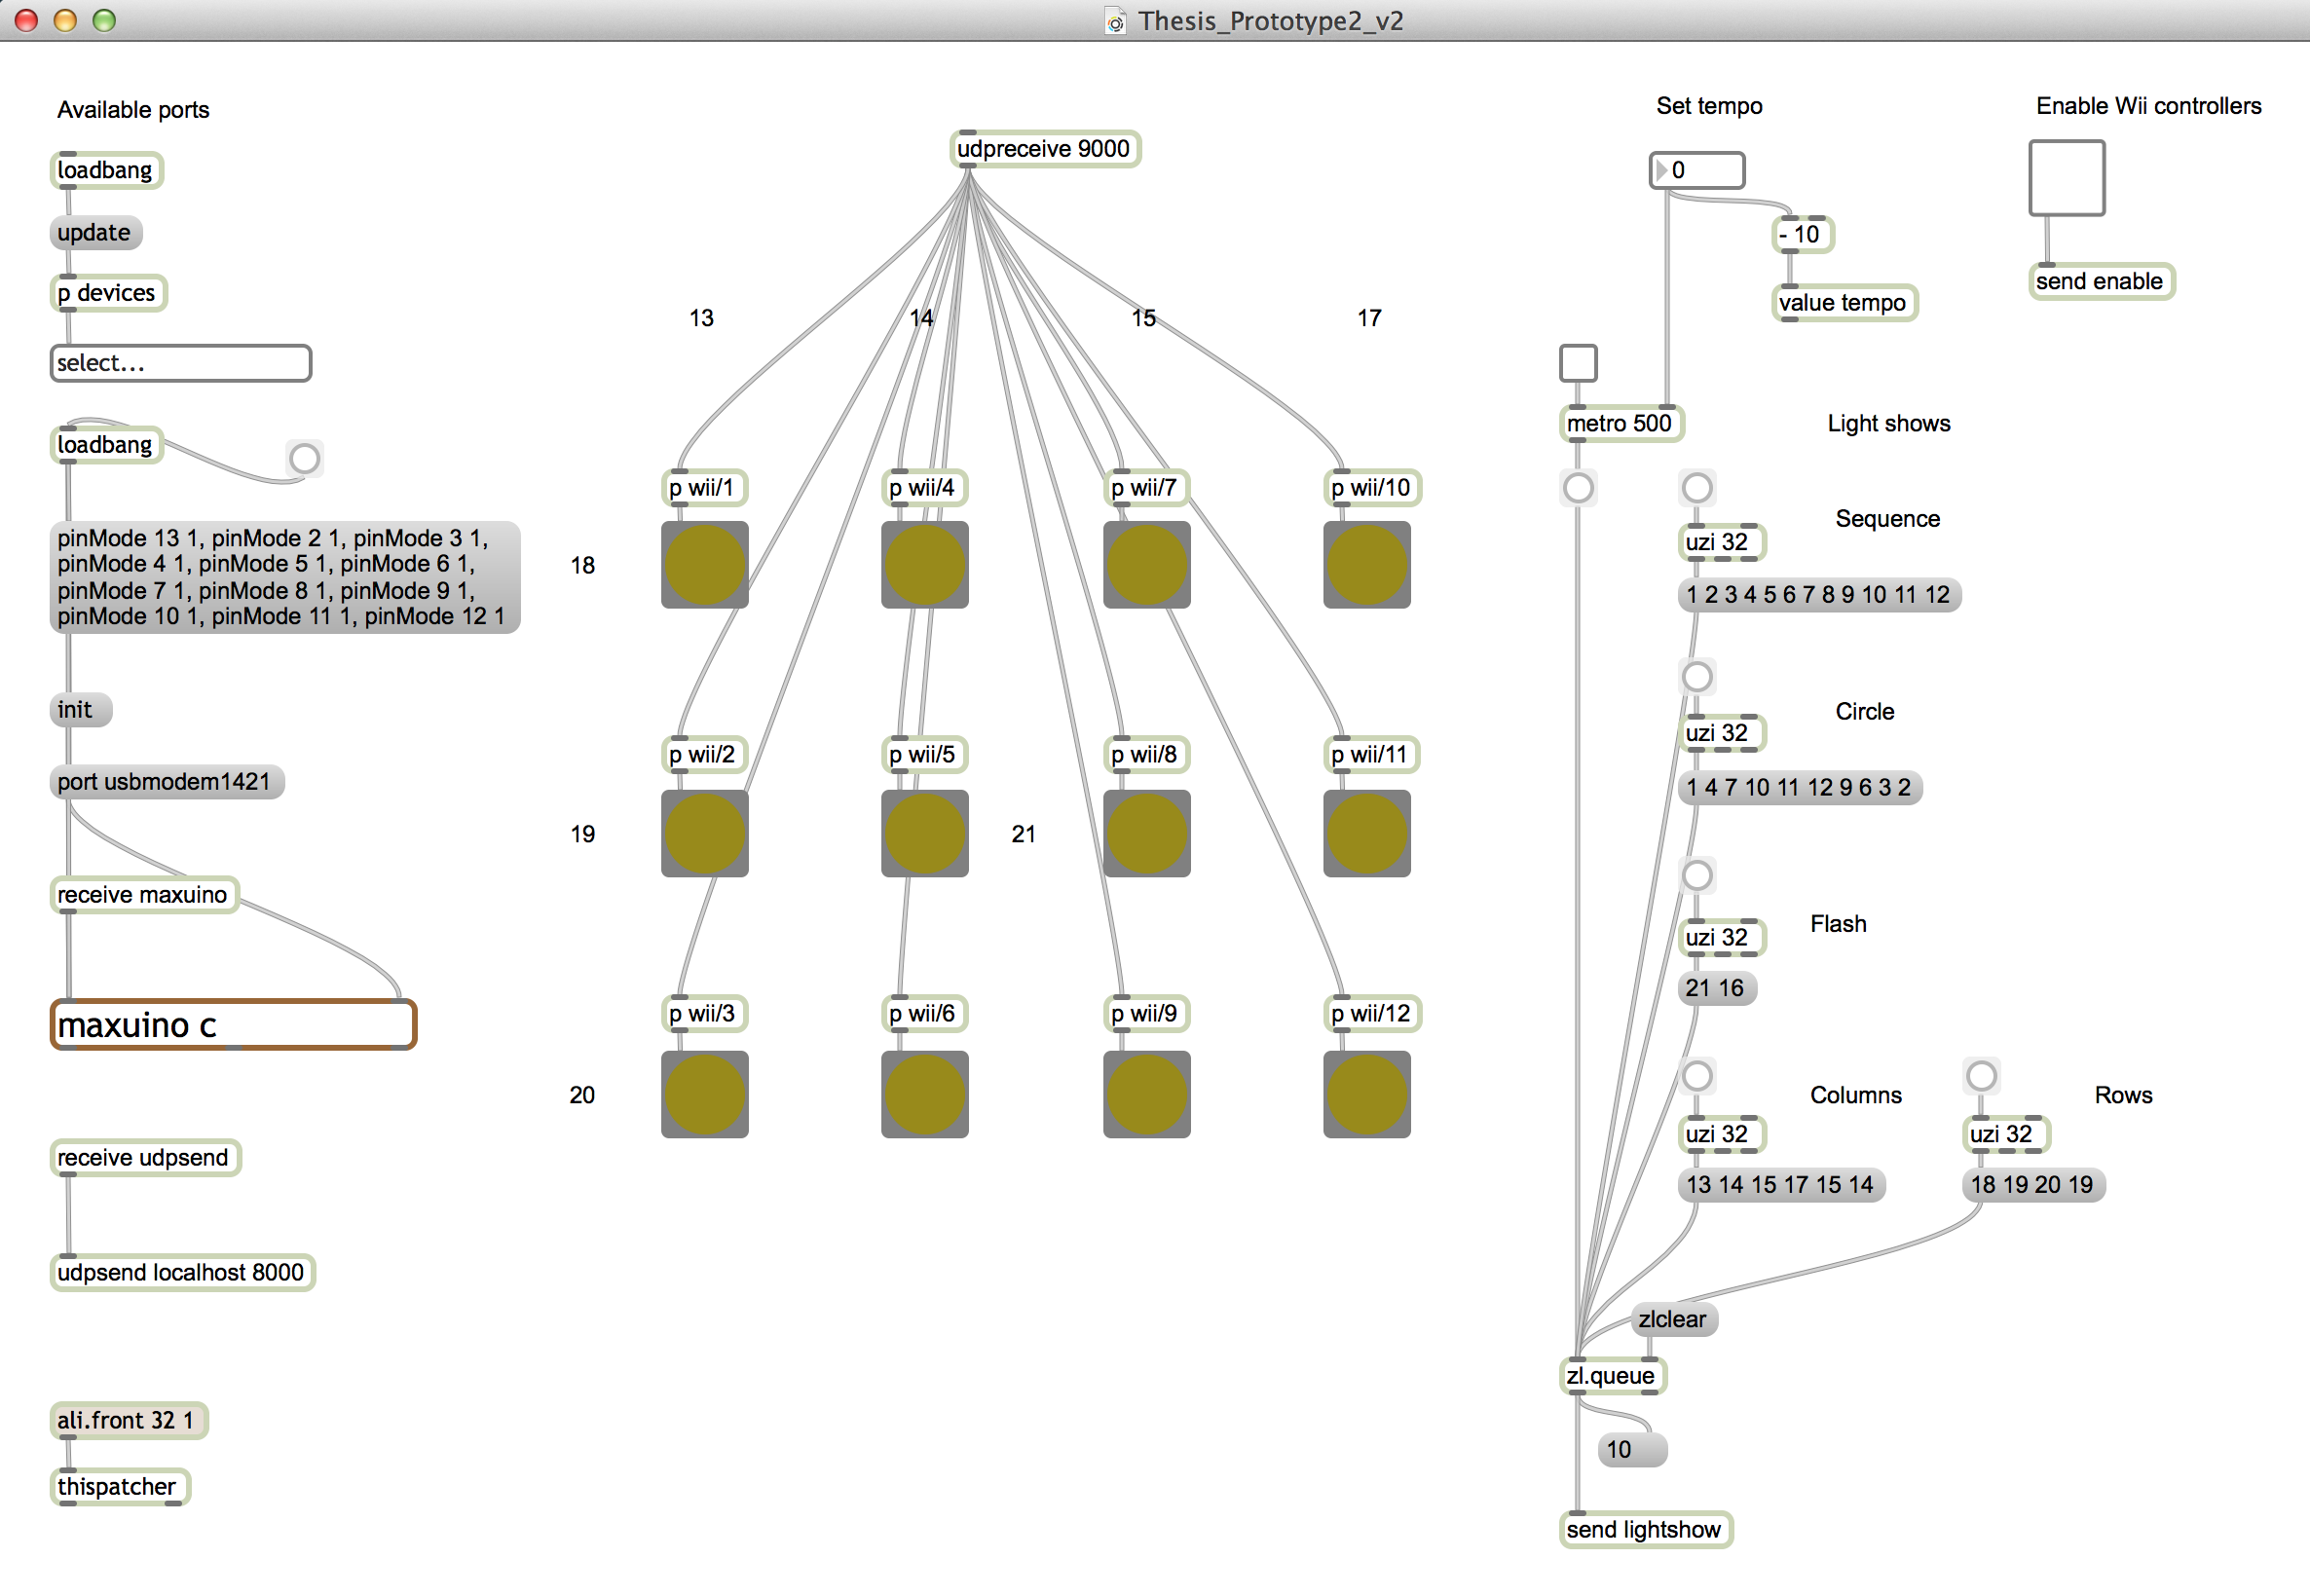
\includegraphics[height=0.4\textwidth]{control.png}
	\caption{Control and monitoring in Max}

	\label{prototyping3.7}
\end{figure}

At this point, discussion with Christian and Molly led to an important question: how long will audience members be controlling these lights? The band and I both felt that the system should not be active for the whole performance; if it caused any unexpected problems, it would be best to not have this affect the entire show. We agreed to introduce the controllers before the band's last two songs. This would give the crowd sufficient time to warm up to the band, and it would serve as a surprising finale. Rather than leaving the lights inactive before this, however, I offered to program a light show to accompany the first part of the performance. Figure \ref{prototyping3.7} shows the Max interface that was designed to control and monitor the lights' activity. For the first part of the show I could trigger preprogrammed lighting patterns, and for the second part I could activate the controllers and oversee audience inputs.

Final adjustments were required to make the system as responsive as possible. This included selecting the threshold for which input values qualified as claps, determining how long a light would remain on for one flash, and fine-tuning a delay to avoid one clap resulting in two consecutive light flashes. As a guide, I tested the values by clapping to the beat of one of Christian Hansen's high-tempo recordings; the values were set when I could do this without the lights flashing too quickly or too slowly.

\subsection{Testing}

\begin{figure}
	\centering

	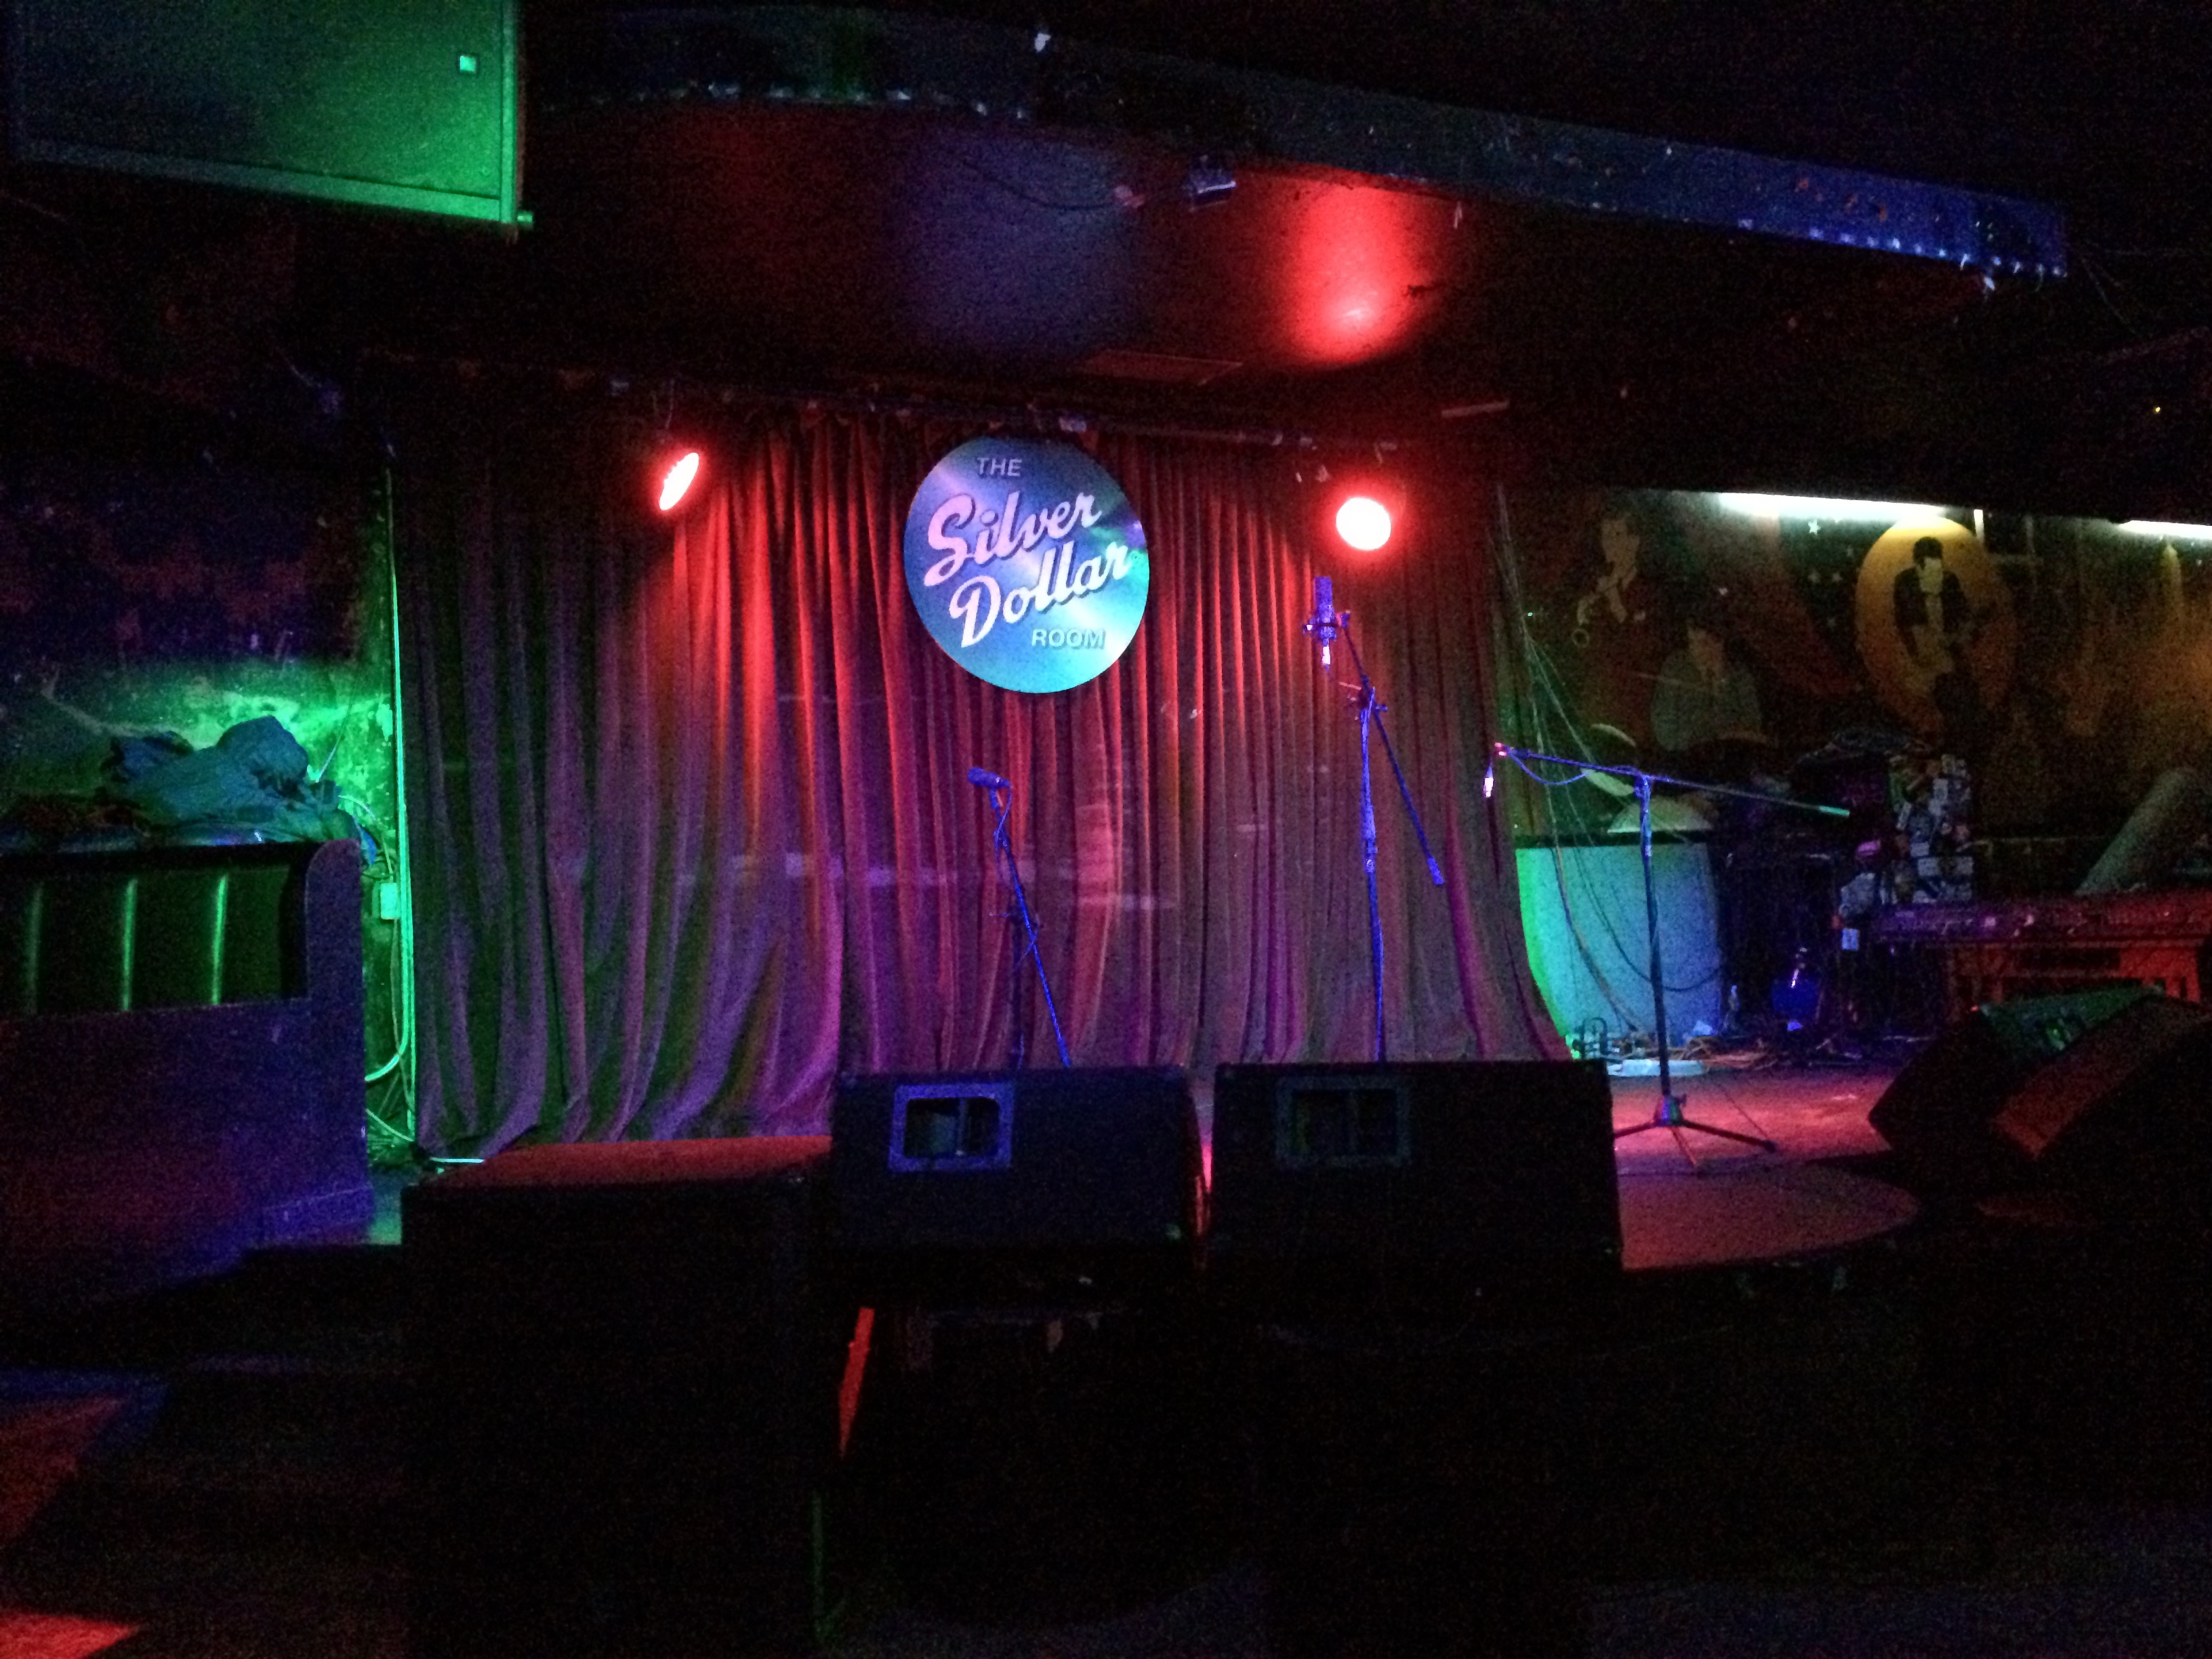
\includegraphics[height=0.4\textwidth]{silver_dollar.jpg}
	\caption{The Silver Dollar Room}

	\label{prototyping3.8}
\end{figure}

The prototype was tested at The Silver Dollar Room, a historic, two-hundred-capacity bar located in downtown Toronto (see Figure \ref{prototyping3.8}). The event took place on a Saturday evening, with Christian Hansen as the headlining act and four other bands on the bill. Christian was scheduled to play for twenty minutes. By the time the band started, the crowd was approximately forty people; Christian guessed that only a fraction of the audience was familiar with his band. The atmosphere was relaxed, most people standing and watching the performers, some with a drink in hand.

\begin{figure}
	\centering

	\includegraphics[height=0.4\textwidth]{lamps.png}
	\caption{Hanging lamps}

	\label{prototyping3.9}
\end{figure}

Due to the number of artists performing, the changeover between sets had to be quick. It was decided that hanging the lights from the keyboard would allow for the simplest setup. Temporary hooks were attached to the keyboard, and the lamps were hung as pictured in Figure \ref{prototyping3.9}. This positioning made the lights sufficiently visible to the crowd. The lamps were plugged in, the Max patcher activated, and the lights all quickly tested in time for the band to begin.

During the performance, I was stationed in a booth directly beside the stage, giving me a clear view of the performers and most audience members. This allowed me to make first-hand observations of the users during the event. Three cameras were also stationed throughout the room to provide video documentation for later reference.

\subsubsection{The Performance}

\begin{figure}
	\centering

	\subfloat{\includegraphics[width=\textwidth]{CH_0.png}}
	\hspace{0.1cm}
	\subfloat{\includegraphics[width=\textwidth]{CH_1.png}}

	\caption{The lights flash as Christian Hansen performs}

	\label{prototyping3.10}
\end{figure}

The performance lasted roughly twenty minutes. For the first part of the show, I was activating preprogrammed lighting patterns, adjusting the speed of the flashing such that it matched the tempo of the song. This worked well; the colour and brightness of the lights suited the environment. Figure \ref{prototyping3.10} shows the band performing with the light show.

With two songs remaining on the set list, Christian announced to the crowd that they were about to run an experiment, announcing, ``We're going to pass control of the lights over to you." Many attendees appeared amused and intrigued. Molly stepped off stage and began passing out Wii controllers to the audience members nearest to the stage. Nobody seemed to hesitate to grab a device. As the participants inspected their controllers, Christian provided a basic explanation of the system. He encouraged users to ``go nuts, get busy, improvise." As users received their controllers, they began clapping, shaking, and flicking the devices and watching the lights react. The lamps flickered erratically. This process of dispersing the controllers and explaining the system took approximately one minute; by the time Christian's explanation was complete, the lamps' flickering had slowed down. Users seemed to understand the concept, and, presumably, most if not all had identified their light. Without wasting any more time, the band launched into their penultimate song ``Please Don't Do That" -- a relatively mellow track, but one with a catchy and consistent beat. The house lights were lowered, and the lamps came to life as users started moving to the music.

\begin{figure}
	\centering

	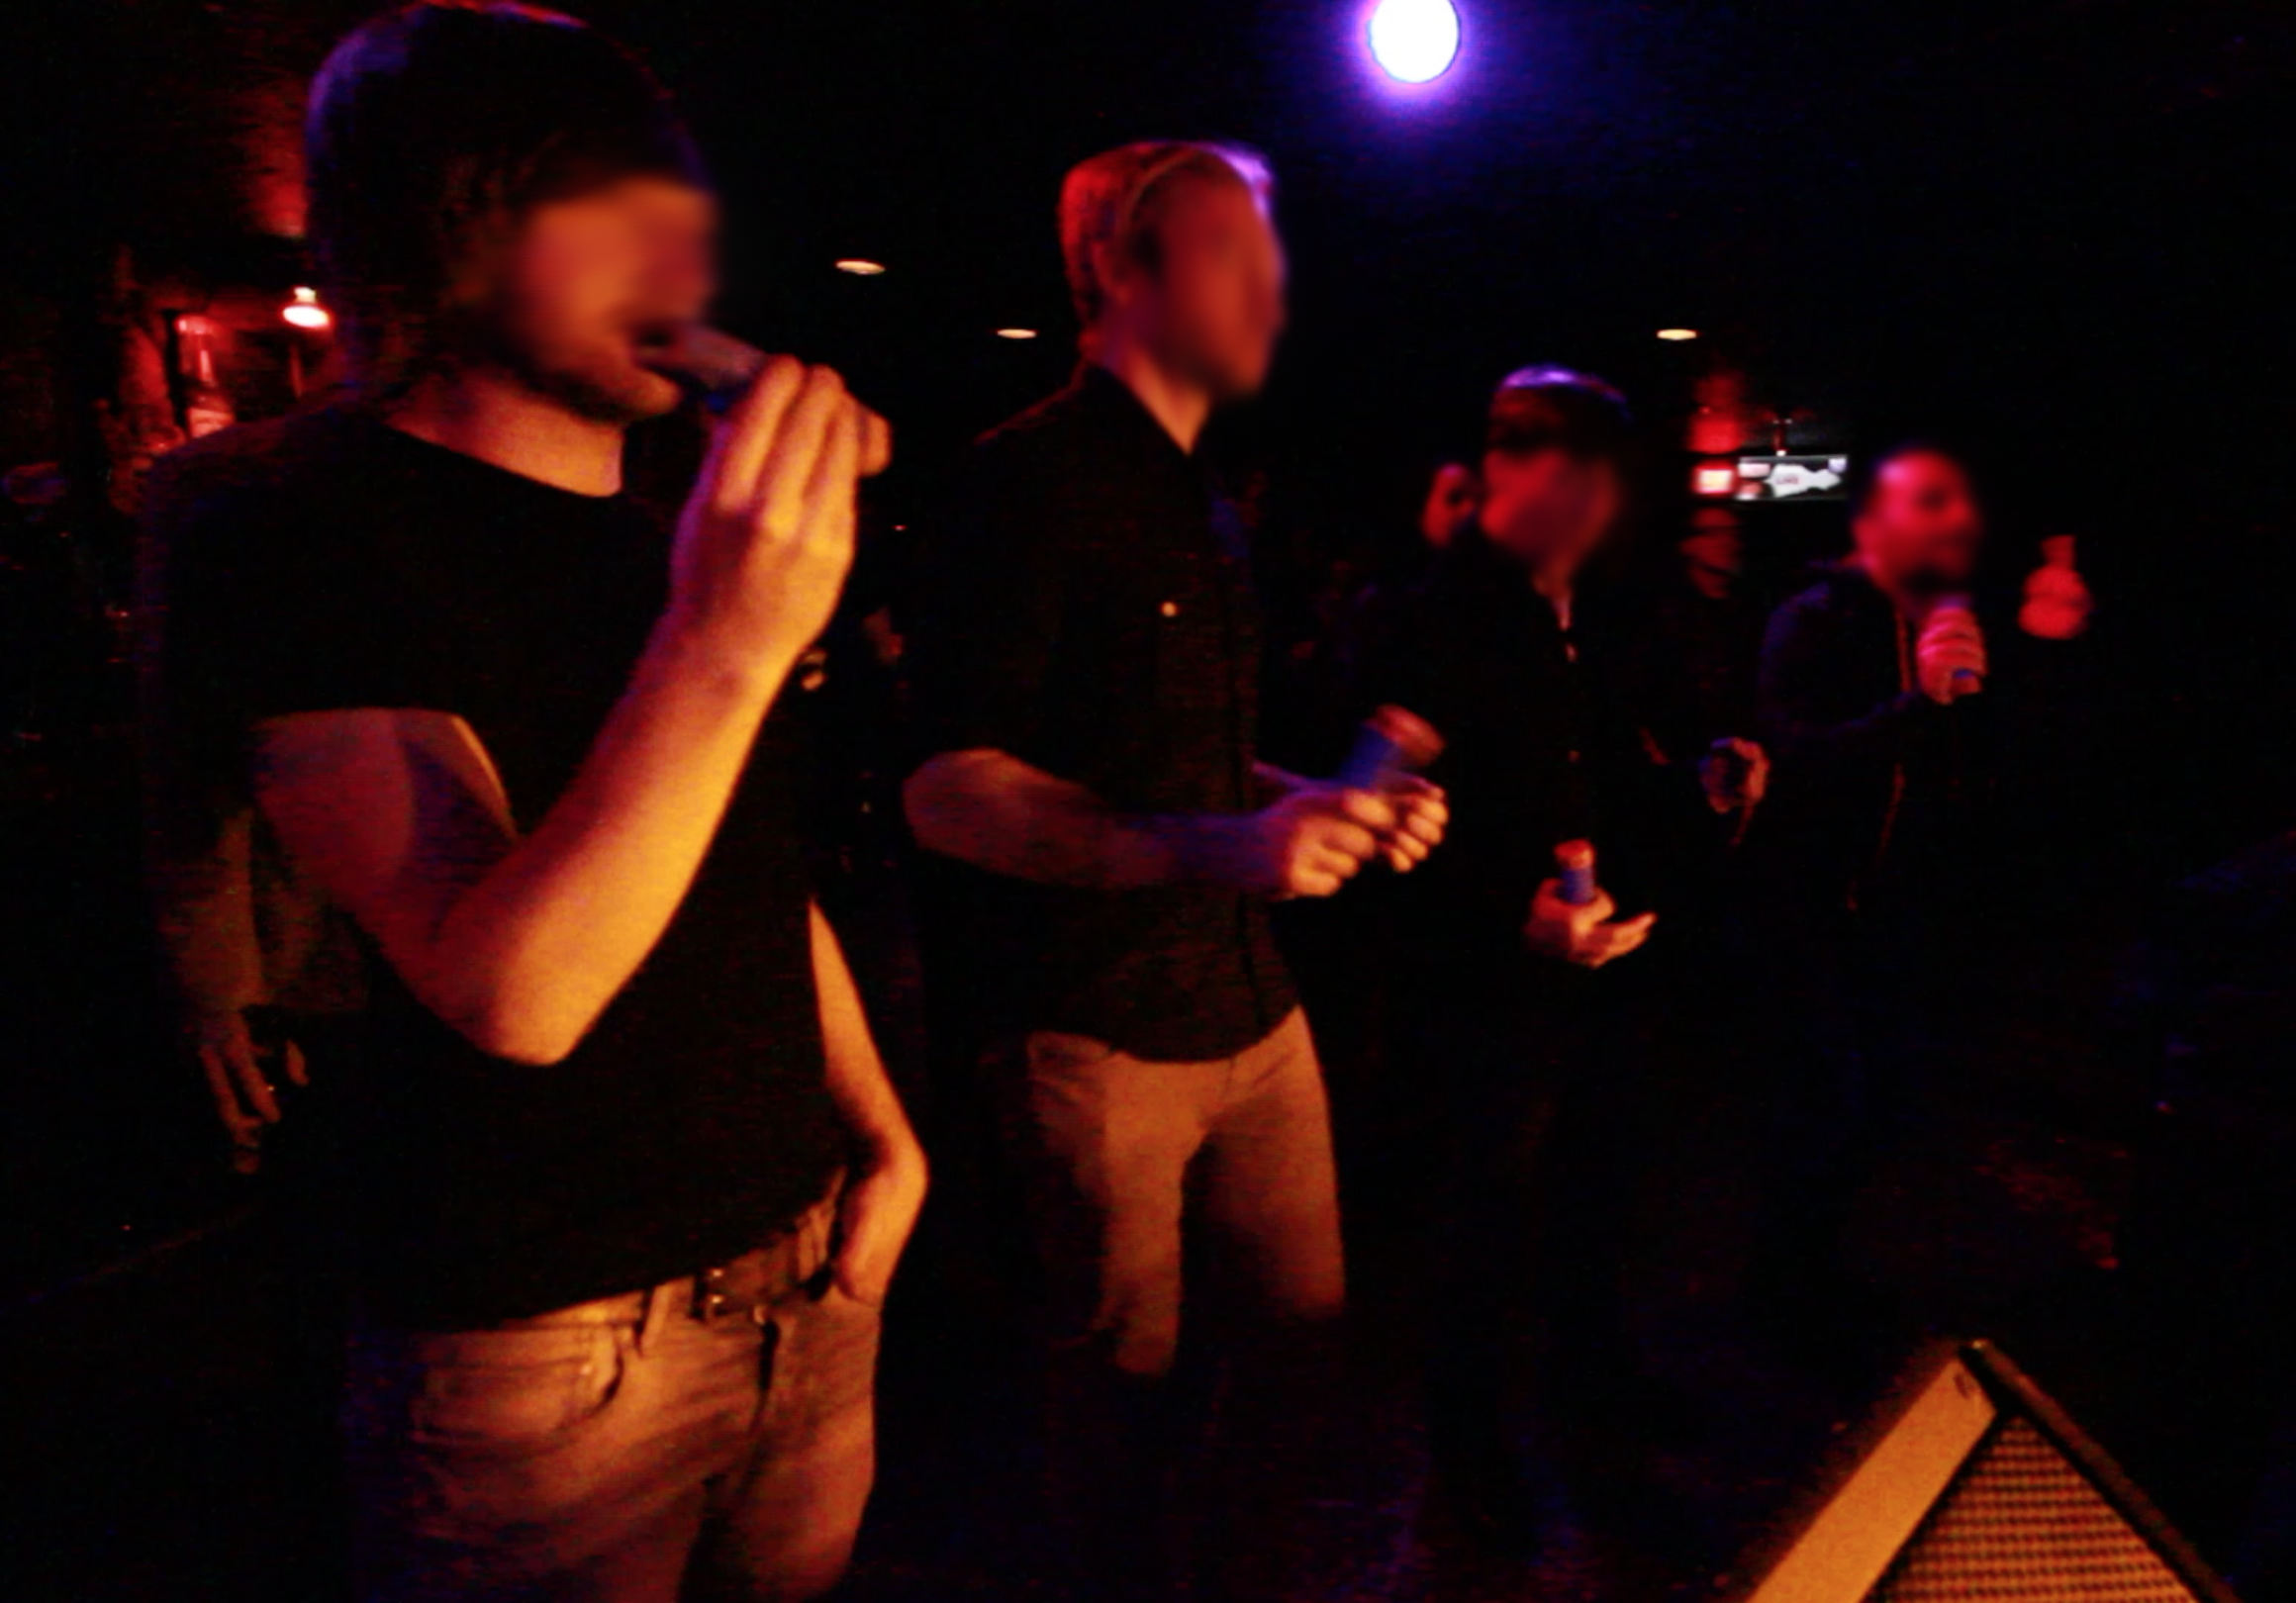
\includegraphics[height=0.4\textwidth]{crowd.png}
	\caption{Audience members move with the controllers}

	\label{prototyping3.11}
\end{figure}

As has been the case with the previous prototypes, the manners in which users handled the devices were surprising. Most held their device as a Wii controller is typically held, the thicker weighted end in their palm; a few others had it flipped upside down. To turn on their light, these users tended to perform a flicking motion -- as if holding a whip or drum stick. One person, in fact, appeared to be `air drumming' to the beat with both hands. Some other users were dancing carelessly, moving their device in random directions at varying speeds. It was unclear how these motions were influencing the lights, but the users did not seem to be paying much attention to the lights. Most surprisingly, there were two participants that held the device from its center, grasping it with the tips of their fingers. One of these people was shaking the device like a shaker, a percussion instrument, for the majority of the performance, and the other was flicking the controller and sometimes twisting it about its center. Notably, there were no users that were consistently performing a clapping motion with their device. While the energy of the crowd was high overall, there were a couple of participants who remained quite still and activated their lights sparingly. There were no users who were noticeably influenced by alcohol. Figure \ref{prototyping3.11} shows four audience members using the controllers.

Audience members also varied in how closely they watched the lights reacting. Initially, of course, users looked closely at the lamps to identify their light. Once this was sorted out, approximately half the users could be observed staring at the lights for portions of the performance; the rest resumed watching the band.

While all participants were moving their controllers along with the music, they were not generally moving in sync with each other. This is because, while some users were activating their light steadily to the beat of the song, others were drumming along with its more complex rhythms. Thus, many of the lights were not flashing at the same time, but most were following the rhythm of the song. The resulting light show, then, appeared random at times but also frequently had moments of cohesion.

\begin{figure}
	\centering

	\subfloat{\includegraphics[width=\textwidth]{CH_2.png}}
	\hspace{0.1cm}
	\subfloat{\includegraphics[width=\textwidth]{CH_3.png}}

	\caption{Christian and Molly interact with the crowd-controlled lamps}

	\label{prototyping3.12}
\end{figure}

As the performance neared its end, it took a surprising turn. Molly took advantage of a vocal-centric part of the song, stepping out from behind her keyboard and pulling two of the lamps off of their hooks. She held them high above her head and shone them on the audience before turning and lighting up Christian's profile. Molly then handed one lamp to her bandmate, and Christian held it in front of himself as he sang the song's closing chorus, the audience-controlled lights illuminating his face. Figure \ref{prototyping3.12} captures these moments.

For the last song of the set, Christian Hansen performed their most popular song, ``Cocaine Trade." This upbeat track kept the audience moving, and nearly all of the lights continued flashing through the end of the song and into the final applause.

\subsubsection{Audience Feedback}

After the performance ended, users returned their device to the table from which I was overseeing the show. Every participant provided a positive comment to me as they handed over their controller (``That was awesome," ``That worked really well"). I spoke briefly to two of the users afterwards to get some more information. Both were in good spirits and did not have any criticisms to offer. They indicated that the system was easy to understand and comfortable to use, and they believed that they knew which light they were in control of. One of the participants who had been dancing frantically through the whole performance explained that it was the band's energy that motivated him to move energetically as well. Interestingly, this person also indicated that this was his first time seeing the band perform; in fact, he had not heard of Christian Hansen before that night.

\subsubsection{Performer Feedback}

I met with Christian one week after the performance, giving him and Molly time to reflect on and discuss the experiment. First, I asked for his overall impressions on the event. ``It was a pretty easy setup. It worked on stage," he said. He indicated that he would like if the lamps had their own stands and could be set up on either side of the stage. He also expressed interest in having some of the lights attached to his microphone. The lights were most effective, he felt, when the venue's house lights were kept low. In general, Christian and Molly had begun thinking about how, logistically, they could tour with this technology and adapt it to different venues.
% They are used to traveling lightly
% Interested in being able to swing the lights around his head
% He saw the technology as an opportunity for something new and exciting to happen. It was ``an added bonus" to their performance.
% He felt that the lamps were most effective when the house lights were kept low.

Once the audience received their controllers, Christian felt that it did not take long for users to understand the technology: ``A minute into the song it was apparent that they knew what they were doing." However, he wondered if the connection could be made more clear -- perhaps by making the output more ``visually significant" or using less lights. Christian believed that the audience had enjoyed the interaction. ``They were engaged with it, but it would be cool to see ... how can the payoff be even bigger for them?" He suggested that the colour of the lights could change in some meaningful way.
% He noted that just being at a concert is satisfying enough for some people.

Christian noted that the show had a ``medium" turnout, and the crowd was a mix of people both familiar and unfamiliar with the band. He explained how different types of shows are handled differently. ``I feel the difference," he said; there are times when it feels right to ask the crowd to participate and times when it does not. If the crowd is onboard, ``you can ask a lot of them and they'll go with you to wherever you want to go."
% He noted that people like options.

There was a particularly memorable moment for Christian when both band members were holding the lamps in their hands: ``It just facilitated something totally new that we've never done before and changed the vibe of the show for sure." He said that using the lights mostly felt natural but for a moment that the band was giving them too much attention. ``You don't want it to become about the light," he warned. He indicated that the occasional randomness of the flashing lights was not a distraction, stating that he ``was ready for that." The only thing that would have been distracted him, he said, was if something malfunctioned.
% ``You don't want it to become about the light. You want it to be a marriage between this awesome light and your face and the music and the whole vibe and story and feeling that it creates."

Christian thought that introducing the devices for the last two songs was a good choice. He felt that giving people control for an entire performance would probably not work out, admitting, ``I don't know if you can expect that much of people." He felt some users were ignoring the lights by the end of the show. He suggested that the rules of the interaction could change periodically throughout the show -- in the same way the mood of the lighting changes in the preprogrammed light shows of major productions. ``For maximum impact ... everything should support the story of the show," he said. The lights could be in the band's control for some parts, in the audience's control for others, or sometimes off altogether; he suggested that some signal could indicate when things change. Christian also proposed that the lights could be moved to different parts of the stage throughout the performance. The band could effectively ``write the script" for where and how the lights illuminate.
% He noted that it makes sense that this [two song interaction] was our instinct

\subsection{Analysis}

Prototype \#3 was an overall success. Every component functioned as expected for the duration of the performance. Ultimately, the testing resulted in several surprising observations of the audience and an insightful discussion with the performer.

The input method was interpreted by users in many different ways. Contrary to expectations, the motions most users were performing were not based on typical audience actions, but at times closely resembled the playing of a percussion instrument. It seems as though the ambiguous form of the device gave people options on how they would like to hold and use it. Designing with ambiguity in this way could promote creativity and give users more freedom; however, one should be sure that unexpected usage does not have adverse effects. The lamps fortunately still responded regardless of the controllers' orientations, but the direction-dependent LEDs, for instance, were rendered meaningless when a user flipped their device upside down or sideways, no longer serving to help them identify their light. This finding brings to mind Turino's (2008) concept of ``wide tuning" in participatory performances; even if participants' behaviours differ, they should all be able to contribute equally.

The concept of audience-controlled lighting was compelling to users overall, but some questions remain unaddressed. For example, this system relies on the participation of each person holding a controller; if most of the users stopped moving, most of the lights would stop flashing, and the effect would diminish. A future iteration could remedy this by adapting to a changing number of participants. It could also reward highly involved users with more control, similar to Feldmeier and Paradiso's (2007) interactive dance club. Previous prototypes were inherently collaborative, implementing many-to-one output and goal-oriented prompts. This iteration, however, did not influence users to collaborate in any way. While the one-to-one mapping connected each audience member with the performance individually, it did not incite communication amongst the crowd. Is this an issue? Is it beneficial for audience members to participate collaboratively, or is it enough that they are contributing to the performance at all? These questions must be addressed in the future.

The instant and direct feedback provided by this prototype seemed to help users quickly understand their role. Christian, however, expressed interest in giving users a ``bigger payoff." Could this be accomplished by using bigger or multicoloured lights? Freeman (2005) stressed that it is impossible to satisfy every member of an audience. Thus, perhaps there is a balance to strike between easy-to-grasp simplicity and a satisfying payoff.
% Instant gratification vs Satisfactory roles
% Freeman, 2005: ``Could the work ever make all 600 audience members feel truly indispensable to its performance? Large-audience participatory works cannot promise instant gratification: giving each person a critical role; requiring no degree of experience, skill, or talent; and creating a unified result which satisfies everyone. Works such as Glimmer reveal the impossibility of this goal even as they strive towards it. They invite participants to explore an environment, discover its limits, and find imaginative ways to express their creativity by pushing against those limits." (4)
% Here is the struggle -- giving users enough control for the interaction to be rewarding but obvious enough feedback that they are confident they are contributing at all

The most appealing aspect of this prototype may have been that it gave the audience some influence over what happened on stage. Rather than creating a network connecting all users together, this system instead created a bridge between those off stage and those on stage. This bridge took the form of the four lamps, which turned into rather compelling artifacts. When the audience had control of the lights and the performers held the lamps in their hands, a new kind of interaction formed. Christian and Molly could direct the lamps and aim them towards the crowd or hold them under their faces, but it was the audience members that chose if and how the lamps were illuminated. The lamps were communal `instruments' that could be `played' by both parties simultaneously. This is tied closely to Bongers' (2000) distinction between reaction and interaction. The lights react to the audience, but ``real interaction" occurred only when the performers began manipulating the lamps as well.

Looking to the future, Christian had expressed interest in making the system more dynamic and able to function for an entire performance. It will be a challenge to create an experience that remains exciting for this amount of time. Implementing different types of inputs or outputs could accomplish this, but is this feasible? Turino (2008) suggests that a main feature of the participatory performance is constancy; would continually changing the system's rules cause too much confusion?
% Story-telling function
% Freeman, 2005: ``Early in the development of Glimmer, a colleague asked me how I would evaluate the piece?s success. I responded that if every audience member believed that the performance would have been different without him or her, then I would be satisfied" (3)
% How can I create the secondary-output version of this? How can the audience feel they are able to influence the performance while keeping the 

% Prototype #3 Outcomes:
% * The lamps were a communal instrument, `played,' albeit in different ways, by both the audience and the performer. Performers are controlling secondary output (lighting). Reactive became Interactive (Bongers).
% * The ambiguous form of the device gave people options on how they'd like to use it
% * Direction-dependent LEDs were rendered meaningless when users flipped the devices upside down or sideways
% * Audience members did not make an attempt to work together. Was this due to attitude or size of the crowd? The fact that a performer was present? A limitation of the technology? Does the one-to-one mapping isolate each user despite the lights being grouped together?
% * This did not really allow for opting out. If half of the participants stood still, for example, would this lessen the effect too much? How can this be remedied?
% * How could different types of interactions be incorporated into the length of a performance? The performer could provide instructions, but is it prohibitive to apply rules to the users? Turino suggests that constancy is a main feature of participatory performance.
% * Alcohol didn't have any noticeable negative effects here